\documentclass[8pt]{beamer}
\usepackage{multirow}
\usepackage{tabulary}
	%\renewcommand{\arraystretch}{1.5}

\usepackage{eurosym} % euro s

\newcommand\Mark[1]{\textsuperscript#1}
\def\res{../res}

%\begin{figure}
%\begin{center}
%\begin{tabular}{cc}
%\resizebox{60mm}{!}{\includegraphics{test1.eps}} &
%\resizebox{60mm}{!}{\includegraphics{test2.eps}} \\
%\resizebox{60mm}{!}{\includegraphics{test3.eps}} &
%\resizebox{60mm}{!}{\includegraphics{test4.eps}} \\
%\end{tabular}
%\caption{This is sample figures.}
%\label{test4}
%\end{center}
%\end{figure}

\usepackage{pgfplots}
\usepackage{filecontents}
\pgfplotsset{compat=newest}
\usepgfplotslibrary{patchplots}
\usepackage{tikz}
\usepackage{pgfplots}
\pgfplotsset{
	table/search path={\res/data/},
}
\usetikzlibrary{backgrounds}
\usetikzlibrary{graphs, graphs.standard, graphdrawing}



\newcommand{\shaded}[1]{\textcolor{gray!30}{#1}}
\usepackage{pifont}
	\newcommand{\ok}{\textcolor{green}{\ding{51}}}
	\newcommand{\ko}{\textcolor{red}{\ding{55}}}

\usepackage{xcolor}
\definecolor{fondtitre}{rgb}{0.20,0.43,0.09}  % vert fonce
\definecolor{coultitre}{rgb}{0.41,0.05,0.05}  % marron
\definecolor{green}{rgb}{0.2,1,0.2}
\definecolor{beamer@blendedblue}{HTML}{404bbf}
\definecolor{violet}{HTML}{5c3566}

\def\blue#1{\textcolor{beamer@blendedblue}{#1}}
\def\violet#1{\textcolor{violet}{#1}}
\def\yellow#1{\textcolor{yellow}{#1}}
\def\red#1{\textcolor{red}{#1}}
\def\green#1{\textcolor{green}{#1}}
\def\black#1{\textcolor{black}{#1}}


\usepackage{color, colortbl}
	\definecolor{mygray}{rgb}{0.5,0.5,0.5}
	\definecolor{mygreen}{rgb}{0,0.6,0}
	\definecolor{gray75}{gray}{0.75}
	\definecolor{marshalcolor}{rgb}{0.93,0.33,0.93} % MARSHAL blue
	\definecolor{draftcolor}{rgb}{0.86,0.86,0.86} % MARSHAL draft color
	\definecolor{darkraspberry}{rgb}{0.53, 0.15, 0.34}


\usepackage{hyperref}
\hypersetup{
%	pdftex,
%	pdfpagemode=FullScreen,
    pdftoolbar=true,        % show Acrobat’s toolbar?
%    pdfborder={0 0 0},
    pdfmenubar=true,        % show Acrobat’s menu?
    pdffitwindow=true,     % window fit to page when opened
    pdfstartview={FitH},    % fits the width of the page to the window
%    pdftitle={title},    % title
%    pdfauthor={Salvatore Mazzarino},     % author
%    pdfsubject={Subject},   % subject of the document
%    pdfcreator={Salvatore Mazzarino},   % creator of the document
%    pdfproducer={Salvatore Mazzarino}, % producer of the document
%    pdfkeywords={Green Networking} {Mobile Cloud} {Network Coding} {Energy}, % list of keywords
    pdfnewwindow=true,      % links in new window
    colorlinks=true,       % false: boxed links; true: colored links
    linkcolor=beamer@blendedblue,          % color of internal links (change box color with linkbordercolor)
    citecolor=beamer@blendedblue,        % color of links to bibliography
    filecolor=beamer@blendedblue,      % color of file links
    urlcolor=beamer@blendedblue           % color of external links
}
    
%    hyperfootnotes=true,
%	breaklinks=true,
%	bookmarksopen=true,
%	backref=page

% sudo apt-get install biber
\usepackage[sorting=none,backref=true,backend=biber, doi=false,url=false,isbn=false, style=numeric]{biblatex}%sorting=nyt, sorting=rasha
%\usepackage[sorting=none,backref=true,backend=biber,sorting=rasha, doi=false,url=false,isbn=false, citetracker,pagetracker=page]{biblatex}%sorting=nyt
	%\setbeamertemplate{bibliography item}{\insertbiblabel}
	%Comme back from citation backref=true
	\addbibresource{/home/aghiles/Aghiles/Redaction/setup/lib/main.bib}
	\addbibresource{/home/aghiles/Aghiles/Redaction/setup/lib/main1.bib}
	\addbibresource{/home/aghiles/Aghiles/Redaction/setup/lib/privacy.bib}
	\def\bibfont{\small}
	\DefineBibliographyStrings{english}{%
		backrefpage = {p.},% originally "cited on page"
		backrefpages = {p.},% originally "cited on pages"
	}
	% Define new format that applies a hypertext reference
	\DeclareFieldFormat{linked}{%
		\ifboolexpr{ test {\ifhyperref} and not test {\ifentrytype{online}}}{
			\iffieldundef{file}{
				\iffieldundef{url}{#1}{\href{run:\thefield{url}}{#1}}
			}{	\href{run:\thefield{file}}{#1}
%				\StrCount{\thefield{file}}{:}[\nbmatch]%
%				\StrCut[\nbmatch]{\thefield{file}}{:}\strfirst\strsecond
%				\StrCount{\strfirst}{:}[\nbmatch]%
%				\StrCut[\nbmatch]{\strfirst}{:}\strfirst\strsecond
%				\href[pdfnewwindow]{run:\strsecond}{#1}
			}
		}{#1}
	}
	% Based on generic definition from biblatex.def
	\renewbibmacro{title}{
		\ifboolexpr{ test {\iffieldundef{title}} }{}{
			\printtext[title]{
				\printtext[linked]{\printfield[titlecase]{title}}
			}
			\newunit
		}
		\printfield{titleaddon}
	}
	%
	\DeclareSourcemap{
	\maps[datatype=bibtex]{
			\map[overwrite=true]{
				\step[fieldsource=groups, fieldtarget=keywords]
			}
		}
	}
	%
%	\DeclareSortingTemplate{rasha}{
%		\sort[direction=ascending]{
%			\field{year}}
%		\sort{\field{presort}}
%	}
	
	\newcommand{\aghiles}[1]{\printbibliography[heading=subbibliography, keyword={#1}, title={#1}]}

%Todo
\newcounter{todo}
\usepackage{tcolorbox}
	\newtcbox{\mytodobox}{colback=white,colframe=white!75!white}
\newcommand\todo[1]{
	\refstepcounter{todo}
	\mytodobox{\hypertarget{todo\thetodo}{#1}}
	\addcontentsline{tod}{subsection}{\protect\hyperlink{todo\thetodo}{\thetodo~#1}\par} }
\makeatletter
\newcommand\listoftodos{
	\@starttoc{tod}}
\makeatother

\usepackage{graphicx}
	\graphicspath{ {\res/} {\res/diagram/} {\res/icon/} {\res/plot/} {\res/stat/} {\res/tikz/} {\res/tmp/}}

\newcommand{\towFigure}[5]{
	\medskip
	\begin{figure}
		\includegraphics[width=#1\columnwidth]{#2} \\
		\includegraphics[width=#1\columnwidth]{#3}
		\caption{#5.}\label{fig:#4}
	\end{figure}
	\medskip
}

\newcommand{\towFigureT}[5]{
	\medskip
	\begin{figure}
		\includegraphics[width=#1\columnwidth]{#2} \\
		\includegraphics[width=#1\columnwidth]{#3}
		\caption*{\blue{Figure} \ref{fig:#4}: #5.}
%		\caption{#5.}\label{fig:#4}
	\end{figure}
	\medskip
}

\newcommand{\Figure}[4]{
	\begin{figure}[#1]
	\centering
	\includegraphics[width=#2\columnwidth]{#3}
	\caption{#4.}\label{fig:#3}
	\end{figure}
}

\newcommand{\Tickz}[4]{
	\medskip
	\begin{figure}[#1]
			\centering
			\begin{tikzpicture}[scale=#2,line width=1pt]
				\input{\res/tikz/#3}
			\end{tikzpicture}
	\caption{#4.}\label{fig:#3}
	\end{figure}
	\medskip
}

\newcommand{\FigureS}[4]{
	\medskip
	\begin{figure}[#1]
	\centering
	\includegraphics[width=#2\columnwidth]{#3}
	\caption*{\blue{Figure \ref{fig:#3}:} #4.}
	\end{figure}
	\medskip
}

\newcommand{\FigureT}[3]{
	\medskip
	\begin{figure}[#1]
	\centering
	\includegraphics[width=#2\columnwidth]{#3}
	\end{figure}
	\medskip
}

\usepackage{subcaption}
	\captionsetup{justification=centering}
%	\captionsetup{labelfont=it,textfont={bf,it},justification=centering}
	
\renewcommand{\thesubfigure}{\alph{subfigure}}
\renewcommand{\thefigure}{\arabic{figure}}

\newcommand{\FigureH}[8]{
%	\medskip
	\begin{figure}
		\centering
		\begin{subfigure}[#1]{#2\columnwidth}
			\centering
			\includegraphics[width=\columnwidth]{#3}
			\caption{#4.}\label{fig:#3}
		\end{subfigure}
		~ % \quad, \qquad, \hfill
		\begin{subfigure}[#1]{#2\columnwidth}
			\centering
			\includegraphics[width=\columnwidth]{#5}
			\caption{#6.}\label{fig:#5}
		\end{subfigure}
		
		\caption{#8.}\label{fig:#7}
	\end{figure}
%	\medskip
}

\newcommand{\FigureV}[8]{
%	\medskip
	\begin{figure}
		\centering
		\begin{subfigure}[#1]{\columnwidth}
			\centering
			\includegraphics[width=#2\columnwidth]{#3}
			\caption{#4.}\label{fig:#3}
		\end{subfigure}
		~ % \quad, \qquad, \hfill
		\begin{subfigure}[#1]{\columnwidth}
			\centering
			\includegraphics[width=#2\columnwidth]{#5}
			\caption{#6.}\label{fig:#5}
		\end{subfigure}
		
		\caption{#8.}\label{fig:#7}
	\end{figure}
%	\medskip
}

\newcommand{\TickzH}[9]{
%	\medskip
	\begin{figure}
	\begin{center}
		\begin{subfigure}[#1]{#2\columnwidth}
			\centering
			\begin{tikzpicture}[scale=#9,line width=1pt]
				\input{\res/tikz/#3}
			\end{tikzpicture}
			\caption{#4.}\label{fig:#3}
		\end{subfigure}
		~ % \quad, \qquad, \hfill
		\begin{subfigure}[#1]{#2\columnwidth}
			\centering
			\begin{tikzpicture}[scale=#9,line width=1pt]
				\input{\res/tikz/#5}
			\end{tikzpicture}
			\caption{#6.}\label{fig:#5}
		\end{subfigure}
		\caption{#8.}\label{fig:#7}
	\end{center}
	\end{figure}
%	\medskip
}

\newcommand{\TickzV}[8]{
%	\medskip
	\begin{figure}
		\centering
		\begin{subfigure}[#1]{\columnwidth}
			\centering
			\begin{tikzpicture}[scale=#2,line width=1pt]
				\input{\res/tikz/#3}
			\end{tikzpicture}
			\caption{#4.}\label{fig:#3}
		\end{subfigure}
		~ % \quad, \qquad, \hfill
		\begin{subfigure}[#1]{\columnwidth}
			\centering
			\begin{tikzpicture}[scale=#2,line width=1pt]
				\input{\res/tikz/#5}
			\end{tikzpicture}
			\caption{#6.}\label{fig:#5}
		\end{subfigure}
		
		\caption{#8.}\label{fig:#7}
	\end{figure}
%	\medskip
}


\newcommand{\Equation}[2]{
	\begin{equation}\label{eq:#1}
		#2
	\end{equation}
}

\newcommand{\EquationT}[2]{
	\begin{equation*}\tag{\ref{eq:#1}}
		#2
	\end{equation*}
}

\newcommand{\EquationS}[1]{
	\begin{equation*}
		#1
	\end{equation*}
}

\newcommand{\Center}[1]{
	\begin{center}
		#1
	\end{center}
}

\newcommand{\Itemize}[1]{
	\begin{itemize}
		#1
	\end{itemize}
}

\newcommand{\Enumerate}[1]{
	\begin{enumerate}
		#1
	\end{enumerate}
}

\newcommand{\Columns}[4]{
	\begin{columns}
		\begin{column}{#1\textwidth}
		#3
		\end{column}
		\begin{column}{#2\textwidth}
		#4
		\end{column}
	\end{columns}
}

\newcommand{\Table}[4]{
	\begin{table}[h!]
		\centering
		\begin{tabulary}{\textwidth}{#1}
			#4
		\end{tabulary}
		\caption{\label{table:#2} #3.}
	\end{table}
}

\newcommand{\TableT}[4]{
	\begin{table}[h!]
	\centering
		\begin{tabular}{#1}
			#4
		\end{tabular}
		\caption*{\blue{Table \ref{table:#2}:~} #3.}
	\end{table}
}

\usepackage{bytefield}
\newcommand{\y}[2]{\bitbox{#1}{#2}}


\usepackage{fourier} % txtbf

\usepackage{hyperref}
% \hypersetup{pdfpagemode=FullScreen}

\setbeamertemplate{bibliography item}{\insertbiblabel}
	
% Beamer
\usetheme{default}
\usecolortheme{default}
\usefonttheme{default}

% Video
\usepackage{multimedia}
\RequirePackage{luatex85}

\usepackage{scrextend}
	\changefontsizes{7.5pt}

%Notes
\usepackage{pgfpages}
\usepackage{palatino}
	\setbeamertemplate{note page}{\pagecolor{lightgray!40}\insertnote}

	\AtBeginNote{
		\hspace*{-20pt}\addtolength\leftmargini{-20pt}
%		\let\itemize\enumerate
%		\let\enditemize\endenumerate
	}
	
%% Foot note
%\makeatletter
%\def\@makefnmark{\hbox{{{%
%	\usebeamercolor[fg]{footnote mark}%
%	\usebeamerfont{footnote mark}%
%	\black{[}\blue{\@thefnmark}\black{]}}%
%}}}
%\def\@makefntext#1{%
%	\def\insertfootnotetext{ #1}%
%	\def\insertfootnotemark{\@makefnmark}%
%	\usebeamertemplate***{footnote}%
%}
%\makeatother

%\setbeamertemplate{bibliography item}{\insertbiblabel}

\makeatletter
\newcommand*{\mkblankfootnote}[1]{%
\begingroup
\renewcommand\thefootnote{}%
\footnotetext{\bibfootnotewrapper{#1}}%
\endgroup
}
\newcommand*{\mkbibsupercite}[1]{%
\def\cbx@savedcites{\cbx@footfullcite}%
%\mkbibsuperscript{\mkbibbrackets{#1}}%
%\blue{\mkbibbrackets{#1}}%
\mkbibbrackets{#1}%
\cbx@savedcites%
}
\DeclareCiteCommand{\supercite}[\mkbibsupercite]
{\gdef\cbx@savedkeys{}}
{\usebibmacro{citeindex}%
\usebibmacro{cite}%
{}%
\xappto\cbx@savedkeys{\thefield{entrykey},}}
{\supercitedelim}
{\protected@xappto\cbx@savedcites{%
[\thefield{prenote}][\thefield{postnote}]{\cbx@savedkeys}}}

\DeclareCiteCommand{\cbx@footfullcite}
{}
{\mkblankfootnote{%
\printtext[labelnumberwidth]{%
\usebibmacro{cite}%
}%
\setunit{\addspace}%
\usedriver
{\DeclareNameAlias{sortname}{default}}
{\thefield{entrytype}}}}
{}
{}
\makeatother

\renewcommand\footcite[1]{\footfullcite{#1}}
%\renewcommand{\thefootnote}{\arabic{footnote}}
\setbeamercolor{footnote}{fg=blue}
\setbeamercolor{footnote mark}{fg=blue}
\setbeamercolor{footline}{fg=blue}
\setbeamercolor{normal text}{fg=black,bg=white}
\setbeamercolor{alerted text}{fg=red}
\setbeamercolor{example text}{fg=green!50!black}
\setbeamercolor{structure}{{fg=beamer@blendedblue}, bg=white}
\setbeamercolor{background canvas}{bg=white}
%\setbeamercolor{page number in head/foot}{fg=blue}

\setbeamerfont{footnote}{size=\tiny}
\setbeamerfont{footline}{series=\bfseries}
%\setbeamerfont{page number in head/foot}{series=\bfseries}

\setbeamertemplate{blocks}[rounded][shadow=true] 
\setbeamertemplate{navigation symbols}{}
\setbeamertemplate{caption}[numbered]
%\setbeamertemplate{footline}[frame number]
%\setbeamertemplate{background canvas}[vertical shading][top=structure.fg!05,bottom=structure.fg!90] 
\setbeamertemplate{section in toc}{\inserttocsectionnumber.~\inserttocsection}
\setbeamertemplate{subsection in toc}{\ \ \ \textcolor{beamer@blendedblue}{\inserttocsubsectionnumber.~\inserttocsubsection} \\}
\setbeamertemplate{frametitle continuation}{}

\setbeamertemplate{itemize item}{\textcolor{blue}{\ding{224}}}
\setbeamertemplate{itemize subitem}{\textcolor{blue}{\ding{223}}}
\setbeamertemplate{itemize subsubitem}{\textcolor{blue}{\ding{84}}}
\setbeamertemplate{itemize subsubsubitem}{\textcolor{blue}{\leadsto}}

%\setbeamertemplate{bibliography item}{\insertbiblabel}

\usepackage{algorithm2e}
\makeatletter
\setbeamertemplate{footline}{
	\leavevmode%
	\hbox{%
	\begin{beamercolorbox}[wd=.75\paperwidth,ht=2.25ex,dp=1ex,left]{author in head/foot}%
		\hspace{1em}
		\ifthenelse{\equal{\@arabic\c@section}{0}}{}{\@arabic\c@section .~\insertsectionhead}
		\ifx
			\insertsubsectionhead\@empty\relax
		\else$\quad\mid\quad$
			\@arabic\c@subsection.~ \insertsubsectionhead
		\fi
		\ifx
			\insertsubsubsectionhead\@empty\relax
		\else$\quad\mid\quad$
			\@arabic\c@subsubsection.~ \insertsubsubsectionhead
		\fi
		%\usebeamerfont{author in head/foot}\insertsection
	\end{beamercolorbox}%
%	\begin{beamercolorbox}[wd=.333333\paperwidth,ht=2.25ex,dp=1ex,center]{title in head/foot}%
%		\usebeamerfont{title in head/foot}\insertsubsection
%	\end{beamercolorbox}%
	\begin{beamercolorbox}[wd=.25\paperwidth,ht=2.25ex,dp=1ex,right]{date in head/foot}%
%		\usebeamerfont{date in head/foot}\insertshortdate{}\hspace*{2em}
		\insertframenumber{} / \inserttotalframenumber\hspace*{2ex} 
	\end{beamercolorbox}}%
	\vskip0pt%
}
\makeatother

\setbeamersize{text margin left=2pt}
\setbeamersize{text margin right=2pt}
\setbeamersize{sidebar width left=2pt}
\setbeamersize{sidebar width right=2pt}

\addtobeamertemplate{navigation symbols}{}{
    \usebeamerfont{footline}%
    \usebeamercolor[fg]{footline}%
    \hspace{1em}%
    %\insertslidenavigationsymbol
	%\insertframenavigationsymbol
	%\insertsubsectionnavigationsymbol
	%\insertsectionnavigationsymbol
	%\insertdocnavigationsymbol
	%\insertbackfindforwardnavigationsymbol
	%\insertframenumber/\inserttotalframenumber
}

\defbeamertemplate{subsubsection in toc}{subsubsections numbered}{
	\leavevmode\leftskip=4.2em
	\normalsize{\rlap{
		\hskip-1.2em \textcolor{beamer@blendedblue}{\inserttocsubsubsectionnumber.}
	}}
	\textcolor{beamer@blendedblue}{\inserttocsubsubsection}\par
}
\setbeamertemplate{subsubsection in toc}[subsubsections numbered]

\defbeamertemplate*{background canvas}{mydefault}{
	\ifbeamercolorempty[bg]{background canvas}{}{\color{bg}\vrule width\paperwidth height\paperheight}
}

\defbeamertemplate*{background canvas}{bg}{
	\color{lightgray!40}\vrule width\paperwidth height\paperheight
}

\BeforeBeginEnvironment{frame}{
	\setbeamertemplate{background canvas}[mydefault]
	\setbeamercolor{frametitle}{bg=white}
}

\makeatletter
\define@key{beamerframe}{bg}[true]{
	\setbeamertemplate{background canvas}[bg]
	\setbeamercolor{frametitle}{bg=lightgray!40}
}
\makeatother

%%%%%%%%%%%%%%%%%%%%%%%%%%%%%%%%%%%%%%%%%%%%%%%%%%%%%%%%%%%%%%%%%%%%%%%%%%%%%

\newcommand{\tableofcontent}{
	\setcounter{tocdepth}{4}
	\setcounter{secnumdepth}{4}
	\begin{frame}[plain,noframenumbering]{Outline}{}
		\begin{columns}
			\begin{column}{0.33\textwidth}
				\setlength{\parindent}{10pt}
				\tableofcontents[sectionstyle=shaded/show,subsectionstyle=hide/hide/hide, subsubsectionstyle=hide/hide/hide]
			\end{column}
			\setbeamertemplate{section in toc shaded}[default][0]
			\begin{column}{0.33\textwidth}
				\tableofcontents[sectionstyle=shaded/hide,subsectionstyle=show/show/hide, subsubsectionstyle=hide/hide/hide]
			\end{column}
			\begin{column}{0.33\textwidth}
				\tableofcontents[sectionstyle=shaded/hide,subsectionstyle=hide/hide/hide, subsubsectionstyle=show/show/hide]
			\end{column}
		\end{columns}
	\end{frame}
}

\newcommand{\transitionsection}{
	\setcounter{tocdepth}{4}
	\setcounter{secnumdepth}{4}
	\begin{frame}[plain,noframenumbering]{Outline}{}
		\begin{columns}
			\begin{column}{0.33\textwidth}
				\setlength{\parindent}{10pt}
				\tableofcontents[sectionstyle=show/shaded,subsectionstyle=hide/hide/hide, subsubsectionstyle=hide/hide/hide]
			\end{column}
			\setbeamertemplate{section in toc shaded}[default][0]
			\begin{column}{0.33\textwidth}
				\tableofcontents[sectionstyle=shaded/hide,subsectionstyle=show/show/hide, subsubsectionstyle=hide/hide/hide]
			\end{column}
			\begin{column}{0.33\textwidth}
				\tableofcontents[sectionstyle=shaded/hide,subsectionstyle=hide/hide/hide, subsubsectionstyle=show/show/hide]
			\end{column}
		\end{columns}
	\end{frame}
}

\newcommand{\transitionsubsection}{
	\setcounter{tocdepth}{4}
	\setcounter{secnumdepth}{4}
	\begin{frame}[plain,noframenumbering]{Outline}{}
		\begin{columns}
			\begin{column}{0.33\textwidth}
				\setlength{\parindent}{10pt}
				\tableofcontents[sectionstyle=show/shaded,subsectionstyle=hide/hide/hide, subsubsectionstyle=hide/hide/hide]
			\end{column}
			\setbeamertemplate{section in toc shaded}[default][0]
			\begin{column}{0.33\textwidth}
				\tableofcontents[sectionstyle=shaded/hide,subsectionstyle=show/shaded/hide, subsubsectionstyle=hide/hide/hide]
			\end{column}
			\begin{column}{0.33\textwidth}
				\tableofcontents[sectionstyle=shaded/hide,subsectionstyle=hide/hide/hide, subsubsectionstyle=show/show/hide]
			\end{column}
		\end{columns}
	\end{frame}
}

\newcommand{\transitionsubsubsection}{
	\setcounter{tocdepth}{4}
	\setcounter{secnumdepth}{4}
	\begin{frame}[plain,noframenumbering]{Outline}{}
		\begin{columns}
			\begin{column}{0.33\textwidth}
				\setlength{\parindent}{10pt}
				\tableofcontents[sectionstyle=show/shaded,subsectionstyle=hide/hide/hide, subsubsectionstyle=hide/hide/hide]
			\end{column}
			\setbeamertemplate{section in toc shaded}[default][0]
			\begin{column}{0.33\textwidth}
				\tableofcontents[sectionstyle=shaded/hide,subsectionstyle=show/shaded/hide, subsubsectionstyle=hide/hide/hide]
			\end{column}
			\begin{column}{0.33\textwidth}
				\tableofcontents[sectionstyle=shaded/hide,subsectionstyle=hide/hide/hide, subsubsectionstyle=show/shaded/hide]
			\end{column}
		\end{columns}
	\end{frame}
}

\AtBeginSection[]{\transitionsection}
\AtBeginSubsection[]{\transitionsubsection}
\AtBeginSubsubsection[]{\transitionsubsubsection}

\usepackage{multicol}
	\newcommand{\alltableofcontent}{
		\begin{frame}[plain,noframenumbering]{Outline}
			\setlength{\parindent}{10pt}
			\begin{multicols}{2}
				\tableofcontents[sectionstyle=show/show,subsectionstyle=show/show/show, subsubsectionstyle=show/show/show]
			\end{multicols}
		\end{frame}
	}

\newcommand{\firstpage}{
	\begin{frame}[plain,noframenumbering]
		\titlepage
			\note[item]{
				Good morning every one, ladies and gentlemen, distinguished guests and supervisors.
				\begin{itemize}
					\item Thank you all for your presence.
					\item ...
				\end{itemize}
			}
		
			\note[item]{My name is DJOUDI Aghiles
				\begin{itemize}
					\item I am a Phd student at Paris-est university and particularly at ESIEE school.
					\item ...
				\end{itemize}
			}
			
			\note[item]{My talk is gonna be on ...
			}
			
			
	\end{frame}
}

\newcommand{\frameBibliography}{
	\newcounter{framenumberappendix}
	\setcounter{framenumberappendix}{\value{framenumber}}

	\begin{frame}[allowframebreaks, plain, noframenumbering]{References}
		\changefontsizes{4pt}
%		\addcontentsline{toc}{chapter}{Bibliography}
		%\printbibheading
		
%		\aghiles{Privacy score}
%		\aghiles{Trust score centrality}
%		\aghiles{Trust score propagation}
%		\aghiles{Trust score capital}
%		\aghiles{Trust score classification}
%		\aghiles{Trust score collaborative}
%		\aghiles{Trust score services}
%		\aghiles{Trust score survey}
%		\aghiles{Trust score visibility}
%		\aghiles{Trust score inference}
%		\aghiles{Trust score divers1}
%		\aghiles{Trust score divers2}
		
		\printbibliography[heading=subbibliography,
%			notkeyword={Privacy score},
%			notkeyword={Trust score centrality},
%			notkeyword={Trust score propagation},
%			notkeyword={Trust score capital},
%			notkeyword={Trust score classification},
%			notkeyword={Trust score collaborative},
%			notkeyword={Trust score services},
%			notkeyword={Trust score survey},
%			notkeyword={Trust score visibility},
%			notkeyword={Trust score inference},
%			notkeyword={Trust score divers1},
%			notkeyword={Trust score divers2},
			title=Others
		]
	\end{frame}

	\addtocounter{framenumberappendix}{-\value{framenumber}}
	\addtocounter{framenumber}{\value{framenumberappendix}} 
}

\newcommand{\bey}[1]{
	\pause
	\begin{tikzpicture}[remember picture, overlay]
		\node[] at (24em, 0ex) {\color{blue!100}\Huge#1};
	\end{tikzpicture}

	% \center{\Huge{Thank you !}}
}

\newcommand{\stamp}[1]{
	\onslide<2->{
	\begin{tikzpicture}[remember picture, overlay]
		\node[draw=red, rotate=30] at (24em, 30ex) {\color{red!90}\huge #1};
	\end{tikzpicture}
	}
}



\usepackage{amsmath}
\usepackage{amssymb}
\usepackage{calc}

\begin{document}

\title{IoT infrastructure}
\subtitle{State of art}
\author{Aghiles DJOUDI}
\institute{Paris-Est University}
%\date{30th September 2014}

\firstpage

\section{Introduction}
	\subsection*{Context}
		\begin{frame}{Context}{Introduction}

\begin{center}

	\begin{figure}
		\includegraphics[width=.7\columnwidth]{res/context.png}
		\caption{\label{fig:context} The IoT Platform}
	\end{figure}
	
\end{center}

\begin{itemize}
	\item Connect sensors to the gateway.
	\item Connect the gateway to the infrastructure.
	\item Store \& Analyze sensors data.
\end{itemize}

	\note{
		\begin{itemize}
			\item Avant de commencer ma présentation, j'aimerai donner un peit apperçu du context de travaille pour ceux qui ne connaissent pas ...
			\item Délimitation du champ de l'étude
			\begin{itemize}
				\item Ce que vous traiterez.
				\item Ce que vous ne traiterez pas.
			\end{itemize}
			\item Voila c'est juste pour vous donner un petit apperçu sur le context
		\end{itemize}
	}

\end{frame}


	\subsection*{Problematic}
		\begin{frame}{Problematic}{Introduction}

\begin{figure}
	\includegraphics[width=.7\columnwidth]{res/iotChallenges.png}
	\caption{\label{fig:iotChallenges}The IoT problematics}
\end{figure}

\begin{itemize}
	\item How to communicate sensors efficiently
		\begin{itemize}
			\item IEEE 802.15.4, 6LowPAN
			\item Throughput, Delay, Jitter, Loss rate and Availability.
		\end{itemize}
	\item How to communicate sensors with the infrastructure efficiently
		\begin{itemize}
			\item LPWAN, LoraWan
			\item Interoperability ?
		\end{itemize}
	\item How to extract knowledge from sensors data.
		\begin{itemize}
			\item Data mining: Classification, Clustering
			\item Deep learning: Machine learning
		\end{itemize}
\end{itemize}
	
	
	\note{
		\begin{itemize}
			\item La manière de poser le problème implique la manière de le résoudre
			\item Savoir ce qui est essentiel de ce qui ne l’est pas.
			\item délimiter un problème
			\item découvrir et rassembler une documentation à son propos
			\item ordonner un contenu
			\item conduire une réflexion personnelle sur le problème choisi
			\item établir des contacts directs avec des personnes, des institutions, des champs d’activités
			\item analyser l’information
			\item exercer son esprit critique
			\item communiquer les résultats de cette procédure d’étude
		\end{itemize}
	}
\end{frame}


%	\subsection*{Motivation}
%		\begin{frame}{Motivation}{Introduction}% What could we win if we resolve this probleme

	\begin{columns}
		\begin{column}{0.5\textwidth}
		
			\begin{itemize}
				\item First motivation
					\begin{itemize}
						\item First motivation
						\begin{itemize}
							\item First motivation
							\item Second motivation
						\end{itemize}
						\item Second motivation
					\end{itemize}
				\item Second motivation
					\begin{itemize}
						\item First motivation
						\item Second motivation
					\end{itemize}
				\item Third motivation
					\begin{itemize}
						\item First motivation
						\item Second motivation
					\end{itemize}
				\item Fourth motivation
					\begin{itemize}
						\item First motivation
						\item Second motivation
					\end{itemize}
			\end{itemize}
			
		\end{column}
	
		\begin{column}{0.5\textwidth}
			\begin{center}
			
				\begin{figure}
					\includegraphics[width=\columnwidth]{res/mail.png}
					\caption{\label{fig:}}
				\end{figure}
				
			\end{center}
		\end{column}
	
	\end{columns}

\note{
	\begin{itemize}
		\item Le sujet est il intéressant à traiter ?
		\item qui va bénificie de la solution et comment
		\item quelle est l'impacte de cette solution sur la varie vie
		\item Motivation pour le choix du sujet
		\item Intérêt du sujet
	\end{itemize}
}

\end{frame}


%	\subsection*{Challenges}
%		\subsection*{Challenges}
% Obstacles, How hard it is, what are the objectifs

\begin{frame}{Challenges}{Introduction}

	\Columns{0.6}{0.4}{
		\Itemize{
			\item Recommend customized security measures
				\Itemize{
					\item New password every time period
					\item Secure the exchange with vulnerable accounts
					\item Adapt permissions to changes
				}
			\item Vulnerability measurement of the social environment
				\Itemize{
					\item Measure the level of vulnerability of interactions
					\item Measure the level of influence between users.
				}
			\item Calculate the vulnerability of the message path
				\Itemize{
					\item Identification of MTA servers
					\item Assign a trust score to each server
					\item Calculate the average confidence of the path.
				}
		}
	}{
		\Figure{!htb}{1}{related.png}{Social interaction}
	}
\end{frame}

\begin{frame}[noframenumbering]{Challenges}{Introduction}

	\Columns{0.6}{0.4}{
		\Itemize{
			\item Recommend customized security measures
				\Itemize{
					\item New password every time period
					\item Secure the exchange with vulnerable accounts
					\item Adapt permissions to changes
				}
			\item \textbf{\blue{Vulnerability measurement of the social environment}}
				\Itemize{
					\item \textbf{\blue{Measure the level of vulnerability of interactions}}
					\item \textbf{\blue{Measure the level of influence between users}}
				}
			\item Calculate the vulnerability of the message path
				\Itemize{
					\item Identification of MTA servers
					\item Assign a trust score to each server
					\item Calculate the average confidence of the path.
				}
		}
	}{
		\FigureS{!htb}{1}{related.png}{Social interaction}
	}
\end{frame}


%	\subsection*{Contributions}
%		\subsection*{Contributions}
% How to overcome these obstacles
% How to verify and validate results ?

\begin{frame}{Contributions}{Introduction}

	\Columns{0.6}{0.4}{
		\Itemize{
			\item Social vulnerability estimation.
				\Itemize{
					\item Individual vulnerability -> Social vulnerability.
					\item Vulnerability diffusion process.
					\item Relationship between trust and vulnerability.
					\item Data: Enron \& Caliopen emails.
				}
		}
	}{
		\Figure{!htb}{0.6}{contagion_revised.jpg}{The vulnerability of one user is the vulnerability of all users}
	}
\end{frame}



\tableofcontent

\section{State of the art}
%	\subsection*{Context}
		\begin{frame}{State of the art}{Standardization}
	
	\note{
		\begin{itemize}
			\item Contenu:
			\begin{itemize}
				\item Tableau comparatif (articles connexes/avantages et désavantages)
				\item Les limites de l’existant
				\item Notre travaille traite le meme x que les travaux précidants mais utilise y au lieu de z (xy/xz)
			\end{itemize}
			\item Procedure:
			\begin{itemize}
				\item Lecture en largeur
				\begin{itemize}
					\item Lecture de beaucoup de papiers connexes
					\item Comprendre le domaine
					\item Comprendre les travaux existants
					\item Sélection des travaux intéressants
				\end{itemize}
				\item Lecture en profondeur
				\begin{itemize}
					\item Lecture et analyse des travaux sélectionnés
					\item Descendre jusqu’au détail du détail
					\begin{itemize}
						\item Poser toujours la question pourquoi?
						\item Être capable d’implémenter de suite l’approche.
					\end{itemize}
				\end{itemize}
				\item Situer le travail par rapport à l’existant sur la base de La problématique traitée
				\begin{itemize}
					\item Les critiques faites sur l’existant
					\item Les hypothèses du travail courant
					\item Les objectifs initiales du travail
					\item Les résultats théoriques et expérimentales obtenus
				\end{itemize}
			\end{itemize}
			\item Article:
			\begin{itemize}
				\item Est-ce que le problème est toujours intéressant ?
				\item Est-ce qu'on peux traiter le problème d'une autre manière ?
				\item Est-ce que les hypothèses sont réalistes ?
				\item Est-ce que le travail est applicable dans le contexte actuel ?
				\item Est-ce que tous les aspects du problème ont été traités ?
				\item Existe-t-il d’autres manières pour le résoudre ?
			\end{itemize}
		\end{itemize}
	}
\end{frame}


	\subsection{Application protocols}
		\begin{frame}{Results}{Comparison with related work}
	\begin{table}
		\begin{tabular}{c|c|c|c|c}
			Paper & A1 & A2 & A3 & A4 \\\hline
				  &    &    &    & \\\hline
				  &    &    &    & \\\hline
				  &    &    &    & \\\hline
				  &    &    &    & 
		\end{tabular}
		\caption{\label{tab:Tableju} An example table.}
	\end{table}
\end{frame}

		\begin{frame}{IoT cloud platforms}{State of the art}
%\changefontsizes{8pt}
\begin{table}[h!]
\begin{center}
	\begin{tabulary}{\textwidth}{L|C|C|C|C}
	\bf{Platform}      & \ \bf{COAP} & \bf{XMPP} & \bf{MQTT}\\\hline
	\bf{Arkessa}       &             &           & \ok      \\\hline
	\bf{Axeda}         &             &           &          \\\hline
	\bf{Etherios}      &             &           &          \\\hline
	\bf{LittleBits}    &             &           &          \\\hline
	\bf{NanoService}   & \ok         &           &          \\\hline
	\bf{Nimbits}       &             & \ok       &          \\\hline
	\bf{Ninja blocks}  &             &           &          \\\hline
	\bf{OnePlateformv} & \ok         & \ok       &          \\\hline
	\bf{RealTime.io}   &             &           &          \\\hline
	\bf{SensorCloud}   &             &           &          \\\hline
	\bf{SmartThings}   &             &           &          \\\hline
	\bf{TempoDB}       &             &           &          \\\hline
	\bf{ThingWorx}     &             &           & \ok      \\\hline
	\bf{Xively}        &             &           & \ok      \\\hline
	\bf{Ubidots}       &             &           & \ok      \\\hline
	
	\end{tabulary}
	\caption{\label{tab:IoTPlatforms} IoT cloud platforms and their characteristics}
\end{center}
\end{table}

\end{frame}


	\subsection{Service discovery}
		\begin{frame}{MDNS}{State of the art}
	\begin{columns}
	
		\begin{column}{0.6\textwidth}
			\begin{itemize}
				\item No need for manual reconfiguration or extra administration
				\item It is able to run without infrastructure
				\item It is able to continue working if failure happens.
				
				\item It inquires names by sending an IP multicast message to all the nodes in the local domain
					\begin{itemize}
						\item Clients asks devices that have the given name to reply back
						\item the target machine receives its name and multicasts its IP @
						\item Devices update their cache with the given name and IP @
					\end{itemize}
				
			\end{itemize}
		\end{column}
		
		\begin{column}{0.4\textwidth}
			\begin{center}
			
				\begin{figure}
					\includegraphics[width=\columnwidth]{mdns.png}
					\caption{\label{fig:mdns} MDNS}
				\end{figure}
				
			\end{center}
			
		\end{column}
	\end{columns}
	
\end{frame}

\begin{frame}{DNS-SD}{State of the art}
	\begin{columns}
		\begin{column}{0.6\textwidth}
		
			\begin{itemize}
				\item Requires zero configuration aids to connect machine
				\item It uses mDNS to send DNS packets to specific multicast addresses through UDP
				\item There are two main steps to process Service Discovery:
					\begin{itemize}
						\item finding host names of required services such as printers
						\item pairing IP addresses with their host names using mDNS
					\end{itemize}
				\item Advantages
					\begin{itemize}
						\item IoT needs an architecture without dependency on a configuration mechanism
						\item smart devices can join the platform or leave it without affecting the behavior of the whole system
					\end{itemize}
				\item Drawbacks
					\begin{itemize}
						\item Need for caching DNS entries
					\end{itemize}
			\end{itemize}
			
		\end{column}
		
		\begin{column}{0.4\textwidth}
			\begin{center}
			
				\begin{figure}
					\includegraphics[width=\columnwidth]{dns-sd.png}
					\caption{\label{fig:dns-sd} DNS-SD}
				\end{figure}
				
			\end{center}
		\end{column}
		
	\end{columns}
	
\end{frame}

\begin{frame}{IoT operating systems}{State of the art}
\changefontsizes{5.3pt}
	\begin{table}[h!]
	\begin{center}
	\begin{tabular}{l|l|c|l|c|c|l|l} % Application protocol
		\bf{OS}      & \bf{Architecture} & \bf{Multi}     & \bf{Scheduling} & \bf{Dynamic}    & \bf{Memory}     & \bf{Network}  & \bf{Virtualization} \\
		\            &                   & \bf{threading} &                 & \bf{Memory}     & \bf{protection} & \bf{Stack} & \bf{and Completion} \\\hline
		\bf{Contiki/Contiki-ng} & Modular        & \ok            & Interrupts      & \ok             & \ko             & uIP          & Serialized          \\
		\            &                   &                & execute w.r.t.  &                 &                 & Rime         & Access              \\\hline
		\bf{MANTIS}  & Modular           & \ko            & Priority        & \ok             & \ko             & At Kernel    & Semaphores.         \\
		\            &                   &                & classes         &                 &                 & COMM layer   &                     \\\hline
		\bf{Nano-RK} & Layered           & \ok            & Monotonic       & \ko             & \ko             & Socket       & Serialized access   \\
		\            &                   &                & harmonized      &                 &                 & abstraction  & semaphores          \\\hline
		\bf{LiteOS}  & Monolithic        & \ok            & Round Robin     & \ok             & \ok             & File         & Synchronization     \\
		\            &                   &                &                 &                 &                 &              & primitives          \\\hline
	\end{tabular}
	\caption{\label{tab:OS} Common operating systems used in IoT environment \cite{al-fuqaha_internet_24}}
	\end{center}
	\end{table}
\end{frame}




	\subsection{Network layer}
		\begin{frame}{IEEE 802.15.4 topologies}{State of the art}
	\begin{columns}
		
		\begin{column}{0.65\textwidth}
		
			\begin{itemize}
			
				\item Standard topologies to form IEEE 802.15.4e networks are 
					\begin{itemize}
						\item[Star] contains at least one FFD and some RFDs
						\item[Mesh] contains a PAN coordinator and other nodes communicate with each other
						\item[Cluster] consists of a PAN coordinator, a cluster head and normal nodes.
					\end{itemize}
					
				\item The IEEE 802.15.4e standard supports 2 types of network nodes
					\begin{itemize}
						\item[FFD] Full function device: serve as a coordinator
							\begin{itemize}
								\item It is responsible for creation, control and maintenance of the net
								\item It store a routing table in their memory and implement a full MAC
							\end{itemize}
						\item[RFD] Reduced function devices: simple nodes with restricted resources
							\begin{itemize}
								\item They can only communicate with a coordinator
								\item They are limited to a star topology
							\end{itemize}
					\end{itemize}
			\end{itemize}
			
		\end{column}
		
		\begin{column}{0.35\textwidth}
			\begin{center}
			
				\begin{figure}
					\includegraphics[width=\columnwidth]{mac.png}
					\caption{\label{fig:topologies} IEEE 802.15.4 topologies. (a) Star. (b) Mesh. (c) Cluster-tree.}
				\end{figure}
				
			\end{center}
		\end{column}
		
	\end{columns}
	
\end{frame}


%		\begin{frame}{RPL protocol}{State of the art}
	\begin{columns}
		
		\begin{column}{0.5\textwidth}
		
			\begin{itemize}
				\item Routing over low-power and lossy links (ROLL)
				\item Support minimal routing requirements.
					\begin{itemize}
						\item like multipoint-to-point, point-to-multipoint and point-to-point.
					\end{itemize}
				\item A Destination Oriented Directed Acyclic Graph (DODAG)
					\begin{itemize}
						\item Directed acyclic graph with a single root.
						\item Each node is aware of ts parents 
						\item but not about related children
					\end{itemize}
				\item RPL uses four types of control messages
					\begin{itemize}
						\item DODAG Information Object (DIO)
						\item Destination Advertisement Object (DAO)
						\item DODAG Information Solicitation (DIS)
						\item DAO Acknowledgment (DAO-ACk)
					\end{itemize}
%				\item RPL routers work under one of two modes:
%					\begin{itemize}
%						\item Non-Storing mode
%						\item Storing modes mode
%					\end{itemize}
			\end{itemize}
			
		\end{column}
		
		\begin{column}{0.5\textwidth}
			\begin{center}
			
				\begin{figure}
					\includegraphics[width=\columnwidth]{rpl.png}
					\caption{\label{fig:rpl} RPL protocol}
				\end{figure}
				
				\begin{figure}
					\includegraphics[width=.3\columnwidth]{rpl2.png}
					\caption{\label{fig:rpl2} DODAG messages}
				\end{figure}
				
			\end{center}
		\end{column}
		
	\end{columns}
	
\end{frame}


%\begin{frame}{Results}{State of the art}
%\changefontsizes{5pt}
%\begin{table}[h!]
%\begin{center}
%	\begin{tabulary}{\textwidth}{L|C|C|C|C|C|C|C|C|C}
%	Paper           & Architecture & Availability & Reliability & Mobility & Performance & Management & Scalability & Interoperability & Security\\\hline
%	IoT-A           &              &              &             &          &             &            &             &                  &         \\\hline
%	IoT@Work        &              &              &             &          &             &            &             &                  &         \\\hline
%	EBBITS          &              &              &             &          &             &            &             &                  &         \\\hline
%	BETaas          &              &              &             &          &             &            &             &                  &         \\\hline
%	CALIPSO         &              &              &             &          &             &            &             &                  &         \\\hline
%	VITAL           &              &              &             &          &             &            &             &                  &         \\\hline
%	SENSAI          &              &              &             &          &             &            &             &                  &         \\\hline

%	RERUM           &              &              &             &          &             &            &             &                  &         \\\hline
%	RELEYonIT       &              &              &             &          &             &            &             &                  &         \\\hline

%	IoT6            &              &              &             &          &             &            &             &                  &         \\\hline
%	OpenIoT         &              &              &             &          &             &            &             &                  &         \\\hline
%	Apec IoV        &              &              &             &          &             &            &             &                  &         \\\hline

%	Smart Santander &              &              &             &          &             &            &             &                  &         \\\hline

%	OMA Device      &              &              &             &          &             &            &             &                  &         \\\hline
%	OMA-DM          &              &              &             &          &             &            &             &                  &         \\\hline
%	LWM2M           &              &              &             &          &             &            &             &                  &         \\\hline
%	NETCONF Light   &              &              &             &          &             &            &             &                  &         \\\hline
%	Kura            &              &              &             &          &             &            &             &                  &         \\\hline
%	MASH            &              &              &             &          &             &            &             &                  &         \\\hline

%	IoT-iCore       &              &              &             &          &             &            &             &                  &         \\\hline
%	PROBE-IT        &              &              &             &          &             &            &             &                  &         \\\hline
%	OpenIoT         &              &              &             &          &             &            &             &                  &         \\\hline
%	LinkSmart       &              &              &             &          &             &            &             &                  &         \\\hline

%	IETF SOLACE     &              &              &             &          &             &            &             &                  &         \\\hline
%	BUTLER          &              &              &             &          &             &            &             &                  &         \\\hline
%	Codo            &              &              &             &          &             &            &             &                  &         \\\hline
%	SVELETE         &              &              &             &          &             &            &             &                  &         \\\hline
%	
%	\end{tabulary}
%	\caption{\label{tab:Table54975} An example table.}
%\end{center}
%\end{table}

%\end{frame}


%	\subsection{Link layer}
	\subsection{Link \& Physical layer}
		\begin{frame}{Results}{State of the art}
\changefontsizes{7pt}
\begin{table}[h!]
\begin{center}
	\begin{tabulary}{\textwidth}{L|L|L|L|L}
	\bf{Phy protocol}  & \bf{Radio band (MHz)} & \bf{MAC address} & \bf{Data rate (bps)} & \bf{Scalability} \\\hline
	\bf{IEEE 802.15.4} & 868/915/2400          & TDMA, CSMA/CA    & 20/40/250 K          & 65K nodes  \\\hline
	\bf{BLE}           & 2400                  & TDMA             & 1024K                & 5917 slaves\\\hline
	\bf{EPCglobal}     & 860-960               & ALOHA            & varies 5-640K        & -          \\\hline
%	\bf{LTE-M}         & 700-900               & OFDMA            & 1G (up), 500M (down) & -          \\\hline
	\bf{Z-Wave}        & 868/908/2400          & CSMA/CA          & 40K                  & 232 nodes  \\\hline
	
	\end{tabulary}
	\caption{\label{tab:IoTPlatforms} IoT cloud platforms and their characteristics \cite{al-fuqaha_internet_24}}
\end{center}
\end{table}

\end{frame}


		\begin{frame}{Results}{Comparison with related work}
\changefontsizes{6pt}
\begin{table}[h!]
\begin{center}
	\begin{tabular}{l|l|l|l}
	\bf{Characteristics}                           & \bf{6LoWPAN}   & \bf{LoRaWAN}                    & \bf{SigFox}  \\\hline
	\bf{Frequency band}                            & 902-929        & 902-928                         & 902          \\
	\bf{\footnotesize{(MHz)}}                      & 868-868.6      & 863-870 and 434                 & 868          \\\hline
	\bf{Number of channels}                        & 0016 for 2400  & 80             for 915          & 25       \\
	\bf{\footnotesize{(channels for MHz)}}         & 0010 for 915   & 10             for 868 and 780  & \\
	\                                              & 0001 for 868.3 &                                 & \\\hline
	\bf{Channel bandwidth}                         & 0005 for 2400  & 0.125 and 0.50 for 915          & 0.0001-0.0012\\
	\bf{\footnotesize{(MHz)}}                      & 0002 for 915   & 0.125 and 0.25 for 868 and 780  & \\
	\                                              & 0600 for 868.3 &                                 & \\\hline
	\bf{Maximum data rate}                         & 0250 for 2400  & 0.00098-0.0219 for 915          & 0.1-0.6      \\
	\bf{\footnotesize{(kbps for MHz)}}             & 0040 for 915   & 0.250-0.05     for 868 and 780  & \\
	\                                              & 0020 for 868.3 &                                 & \\\hline
%	\bf{Channel modulation}                       & QPSK for 2400  & LoRa           for 915          & BPSK and GFSK\\
%	\                                             & BPSK for 915   & LoRa and GFSK  for 868  and 780 & \\
%	\                                             & BPSK for 868.3 &                                 & \\\hline
	\bf{Channel coding}                            & -085 for 2400  & -137                            & -137         \\
	\bf{\footnotesize{(dBm for MHz)}}              & -092 for 915   &                                 & \\
	\                                              & -092 for 868.3 &                                 & \\\hline
	\bf{Protocol data unit \footnotesize{(bytes)}} & 6+127          & x + (19 to 250)                 & 12+ (0 to 12)\\\hline
	\bf{Channel coding}                            & Direct         & CSS                             & Ultra        \\\hline
	\bf{Transmission range}                        & 10-100 m       & 5-15 km                         & 10-50 km     \\\hline
	\bf{Battery lifetime}                          & 1-2 years      & <10 years                       & <10 years    \\\hline

	\end{tabular}
	\caption{\label{tab:Table54975} LPWan Characteristics \cite{al-kashoash_comparison_2016}}
\end{center}
\end{table}

\end{frame}


%\begin{frame}{Results}{Comparison with related work}
%\changefontsizes{7pt}
%\begin{table}[h!]
%\begin{center}
%	\begin{tabulary}{\textwidth}{L|L|L|L|L|L}
%	\bf{Feature}                     & \bf{Wi-Fi}                                            & \bf{802.11p}                                          & \bf{UMTS}                        & LTE                      & LTE-A                     \\\hline
%	\bf{Channel width MHz}           & 20                                                    & 10                                                    & 5                                & 1.4, 3, 5, 10, 15, 20    & Up to 100                 \\\hline
%	\bf{Frequency band(s) GHz}       & 2.4 , 5.2                                             & 5.86-5.92                                             & 0.7-2.6                          & 0.7-2.69                 & 0.45-4.99                 \\\hline
%	\bf{Bit rate Mb/s}               & 6-54                                                  & 3–27                                                  & 2                                & Up to 300                & Up to 1000                \\\hline
%	\bf{Range km}                    & Up to 0.1                                             & Up to 1                                               & Up to 10                         & Up to 30                 & Up to 30                  \\\hline
%	\bf{Capacity}                    & Medium                                                & Medium                                                & \ko                              & \ok                      & \ok                       \\\hline
%	\bf{Coverage}                    & Intermittent                                          & Intermittent                                          & Ubiquitous                       & Ubiquitous               & Ubiquitous                \\\hline
%	\bf{Mobility support km/h}       & \ko                                                   & Medium                                                & \ok                              & up to 350                & up to 350                 \\\hline
%	\bf{QoS support}                 & EDCA \scriptsize{Enhanced Distributed Channel Access} & EDCA \scriptsize{Enhanced Distributed Channel Access} & QoS classes and bearer selection & QCI and bearer selection & QCI and bearer selection  \\\hline
%	\bf{Broadcast/multicast support} & Native broadcast                                      & Native broadcast                                      & Through MBMS                     & Through eMBMS            & Through eMBMS             \\\hline
%	\bf{V2I support}                 & \ok                                                   & \ok                                                   & \ok                              & \ok                      & \ok                       \\\hline
%	\bf{V2V support}                 & Native (ad hoc)                                       & Native (ad hoc)                                       & \ko                              & \ko                      & Through D2D               \\\hline
%	\bf{Market penetration}          & \ok                                                   & \ko                                                   & \ok                              & \ok                      & \ok                       \\\hline

%	\end{tabulary}
%	\caption{\label{tab:Tableppp} An example table.}
%\end{center}
%\end{table}

%\end{frame}

%\begin{frame}{Results}{Comparison with related work}
%\changefontsizes{7pt}
%\begin{table}[h!]
%\begin{center}
%	\begin{tabulary}{\textwidth}{L|L|L|L|L|L}
%	\bf{Feature}                     & \bf{RFID}                                            & \bf{ZigBee}                                          & \bf{NFC}                        & LTE                      & LTE-A                     \\\hline
%	\bf{Channel width MHz}           & 20                                                    & 10                                                    & 5                                & 1.4, 3, 5, 10, 15, 20    & Up to 100                 \\\hline
%	\bf{Frequency band(s) GHz}       & 2.4 , 5.2                                             & 5.86-5.92                                             & 0.7-2.6                          & 0.7-2.69                 & 0.45-4.99                 \\\hline
%	\bf{Bit rate Mb/s}               & 6-54                                                  & 3–27                                                  & 2                                & Up to 300                & Up to 1000                \\\hline
%	\bf{Range m}                     & 3-10                                                  & 10-100                                                & Up to 6.1                         & Up to 30                 & Up to 30                  \\\hline
%	\bf{Capacity}                    & Medium                                                & Medium                                                & \ko                              & \ok                      & \ok                       \\\hline
%	\bf{Coverage}                    & Intermittent                                          & Intermittent                                          & Ubiquitous                       & Ubiquitous               & Ubiquitous                \\\hline
%	\bf{Mobility support km/h}       & \ko                                                   & Medium                                                & \ok                              & up to 350                & up to 350                 \\\hline
%	\bf{QoS support}                 & EDCA \scriptsize{Enhanced Distributed Channel Access} & EDCA \scriptsize{Enhanced Distributed Channel Access} & QoS classes and bearer selection & QCI and bearer selection & QCI and bearer selection  \\\hline
%	\bf{Broadcast/multicast support} & Native broadcast                                      & Native broadcast                                      & Through MBMS                     & Through eMBMS            & Through eMBMS             \\\hline
%	\bf{V2I support}                 & \ok                                                   & \ok                                                   & \ok                              & \ok                      & \ok                       \\\hline
%	\bf{V2V support}                 & Native (ad hoc)                                       & Native (ad hoc)                                       & \ko                              & \ko                      & Through D2D               \\\hline
%	\bf{Market penetration}          & \ok                                                   & \ko                                                   & \ok                              & \ok                      & \ok                       \\\hline
%	\bf{Data rate}                   & Up to 640 kbps                                        & 250 kbps                                              & 106–424 kbps                              & \ok                      & \ok                       \\\hline
%	\end{tabulary}
%	\caption{\label{tab:Tabliutecv} An example table.}
%\end{center}
%\end{table}

%\end{frame}



%\begin{frame}{Results}{Comparison with related work}

%%\begin{table}[h!]
%%\begin{center}
%	\begin{tabulary}{\textwidth}{|C|C|C|C|C|C|C|C|C|}\hline
%		Preamble & PHDR & PHDRCRC & MHDR & FHDR & FPort & Payload & MIC & CRC \\\hline
%	\end{tabulary}
%%	\caption{\label{tab:Tableijkiikk} An example table.}
%%\end{center}
%%\end{table}

%\end{frame}


%\begin{frame}{Use cases}{Comparison with related work}
%%\changefontsizes{5pt}
%\begin{table}[h!]
%\begin{center}
%	\begin{tabular}{l|l|l|l}
%	\textbf{Use cases}         &  &  & \\\hline
%	Health Monitoring          &  &  & \\\hline
%	Water Distribution         &  &  & \\\hline
%	Electricity Distribution   &  &  & \\\hline
%	Smart Buildings            &  &  & \\\hline
%	Intelligent Transportation &  &  & \\\hline
%	Surveillance               &  &  & \\\hline
%	Environmental Monitoring   &  &  & \\
%	\end{tabular}
%	\caption{\label{tab:IoTUseCase} Use cases \cite{hancke_role_2012}}
%\end{center}
%\end{table}

%\end{frame}


%	\subsection{Contagion process}
%%		\subsection{Contagion process}
\begin{frame}{... (step 1)}{Methods}

\Itemize{
	\item S = {SF12, BW125, 4/8, 17 dBm}
	\item Input: 
	\Itemize{
		\item Problem: f(x) = {max($x^{2}$), x \in [0,32]}
		\Itemize{
			\item $x_{1}: 01101_{b}$ 
			\item $x_{2}: 11000_{b}$
			\item $x_{3}: 01000_{b}$
			\item $x_{4}: 10011_{b}$
		}
	}

	\item Method: Genetic algorithm
	\Itemize{
		\item Generate a set of random possible solution
		\item Test each solution and see how good it is (ranking)
		\Enumerate{
			\item Remove some bad solutions
			\item Duplicate some good solutions
			\item Make small changes to some of them (Crossover, Mutation)
		}
	}

	\item Output:
	\Itemize{
			\item $x_{1}$: 01101  (169)  (14.4)
			\item $x_{2}$: 11000  (576)  (49.2)
			\item $x_{3}$: 01000  (64 )  (5.5)
			\item $x_{4}$: 10011  (361)  (30.9)
	}
}
\end{frame}

%\note{
%	\begin{itemize}
%		\item Contenu:
%		\begin{itemize}
%			\item L’approche doit être soigneusement détaillée
%			\item Motiver les étapes, les hypothèses, le contexte
%			\item Dérouler un exemple si nécessaire
%			\item Illustrer par des schémas et figures
%			\item Se concentrer sur les aspects où l’approche apporte une contribution
%			\item Montrer comment on est différent de l’existant
%		\end{itemize}
%		\item Conseils:
%		\begin{itemize}
%			\item Présentation de l'approche utilisée pour résoudre le problème posé: approche(contrainte, parametre du probleme) = solution
%			\begin{itemize}
%				\item Justification du choix de l'approche
%				\item Description générale de l’approche comme une boite noir
%				\begin{itemize}
%					\item Entrées, Sorties, Contraintes, Hypothèses
%				\end{itemize}
%				\item Description détaillée de la solution du problème
%				\begin{itemize}
%					\item Description détaillée des étapes: paramètre -> étape1 -> étape2, ... -> solution
%					\item Modélisation des objets manipulés
%				\end{itemize}
%			\end{itemize}
%			\item Mise en œuvre des hypothèses
%			\item Description de la solution du problème
%		\end{itemize}
%		\item Conseils 2:
%		\begin{itemize}
%			\item Utilisez un exemple pour le dérouler tout au long des étapes de l’approche
%			\item Ne parlez dans ce chapitre que de votre travail, ce qu’ont fait les autres est dans l’état de l’art
%			\item Insistez sur les parties où vous apportez des contributions
%			\item Montrez comment votre travail est différent des autres
%			\item Montrez les modules/algorithmes pris de l’existant, ne réinventez pas la roue.
%			\item le lecteur doit pouvoir reproduire les résultats en appliquant la même approche.
%		\end{itemize}
%	\end{itemize}
%}

\begin{frame}{... (step 2)}{Methods}
	\Itemize{
		\item 
		\item 
	}
\end{frame}

\begin{frame}{... (step 3)}{Methods}
	\Itemize{
		\item 
		\item 
	}
\end{frame}

\begin{frame}{... (step 4)}{Methods}
	\Itemize{
		\item 
		\item 
	}
\end{frame}

\begin{frame}{Results}{Comparison}
	\begin{table}[h!]
	\scriptsize
		\begin{tabulary}{\textwidth}{L|L|L|L|L}
		\  &  &  &  &  \\\hline
		\  &  &  &  &  \\\hline
		\  &  &  &  &  \\\hline
		\  &  &  &  &  \\\hline
		\  &  &  &  &  \\\hline
		\end{tabulary}
	\caption{\label{tab:} }
	\end{table}
\end{frame}


%	\subsection{Experimentation}
%		\subsection{Experimentation}
\begin{frame}{Experimentation}{Experimentation}
	\begin{itemize}
		\item Privacy threats
			\begin{itemize}
				\item Privacy settings
				\item Information propagation
				\item 
			\end{itemize}
		\item Privacy protection
			\begin{itemize}
				\item Privacy settings
				\item I
			\end{itemize}
	\end{itemize}
	
\end{frame}


%	\subsection{Results exploitation}
%		\subsubsection{Context}
%		\subsubsection{Context}
%		\begin{frame}{Results}{Comparison}

	\Columns{0.5}{0.5}{
		\begin{figure}
			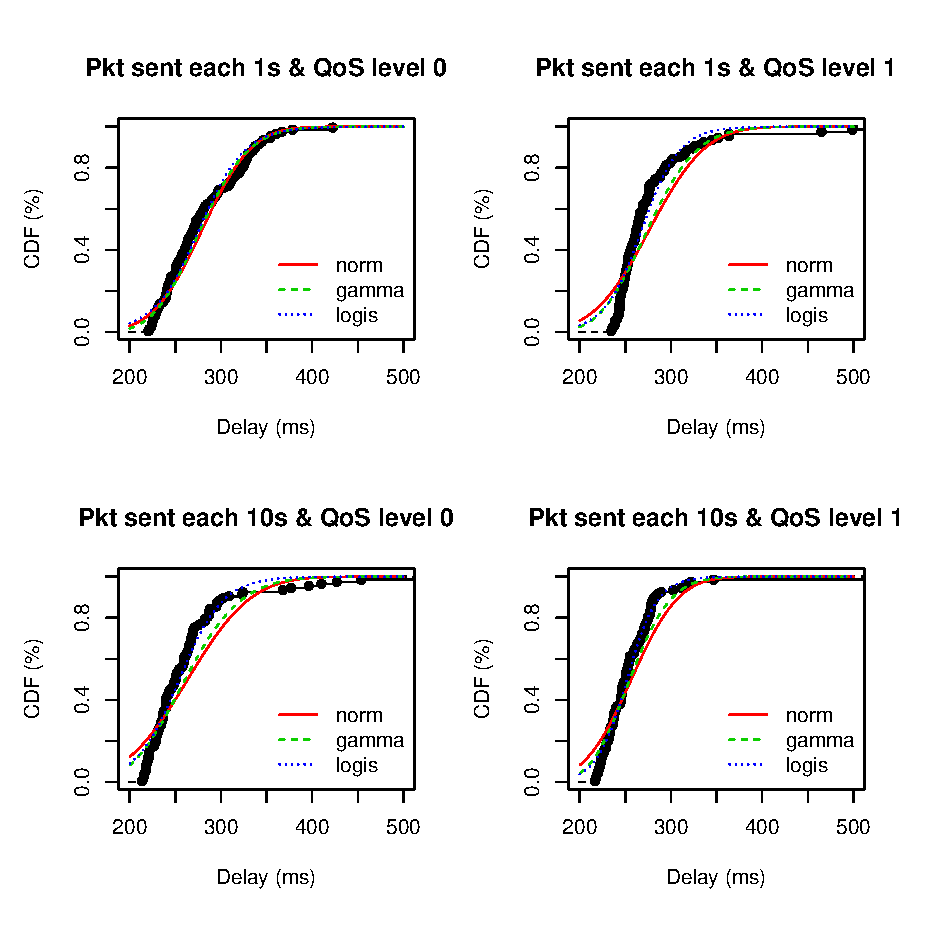
\includegraphics[width=\columnwidth]{distributions_v3.eps}
			\caption{\label{fig:distributions_v3.eps}Distributions}
		\end{figure}
	}{
		\begin{figure}
			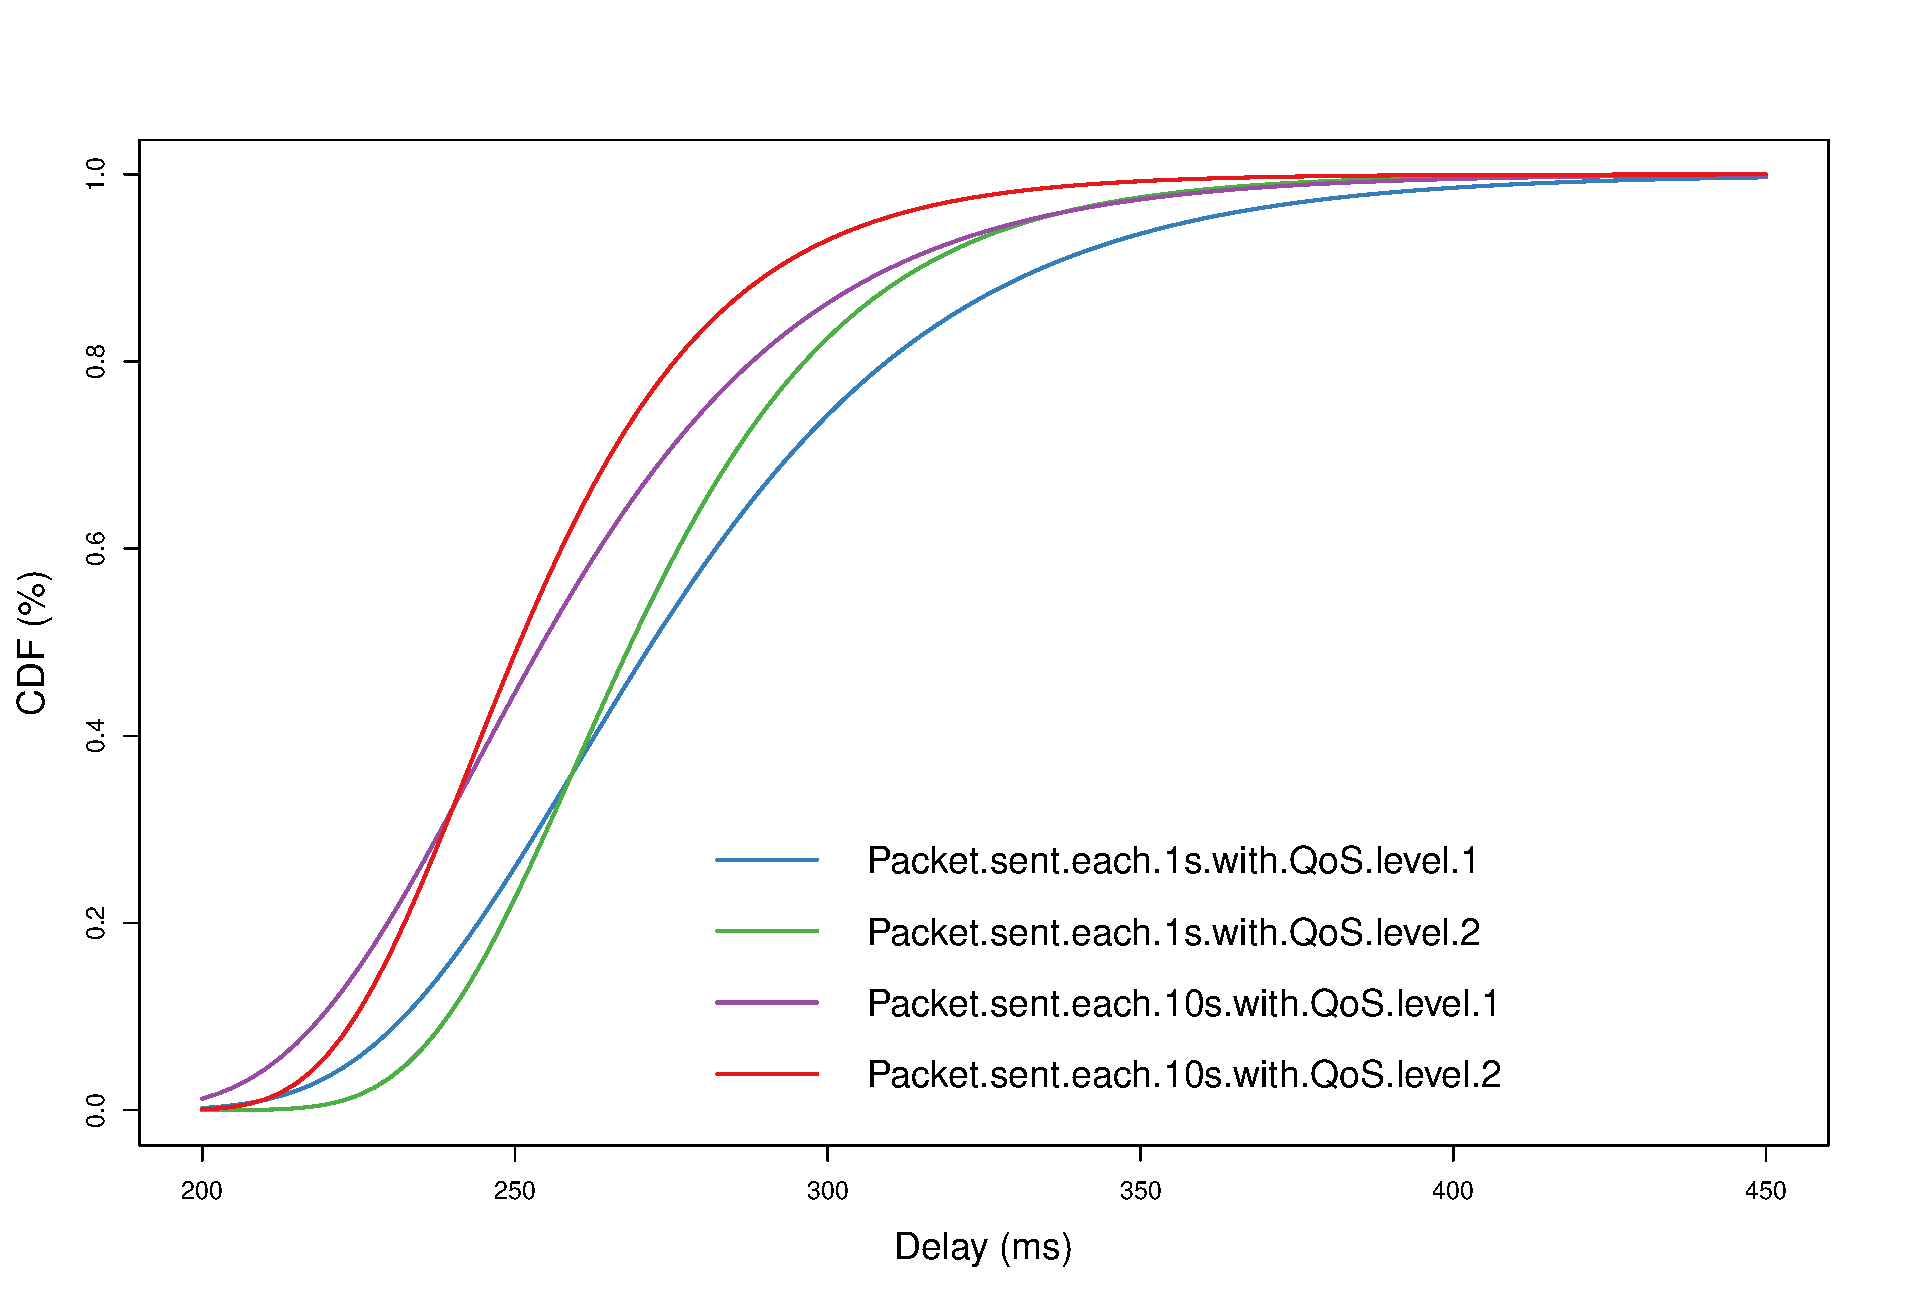
\includegraphics[width=\columnwidth]{res/cdf_v3.eps}
			\caption{\label{fig:cdf_v3.eps}CDF comparison}
		\end{figure}
	}
	
\end{frame}


%	\subsection{Conclusion}
%		\subsection{Conclusion}
\begin{frame}{Conclusion}

	\begin{columns}
		\begin{column}{0.5\textwidth}
%			\newcolumntype{a}{>{\columncolor[gray]{0.8}}c}
			\begin{figure}
				\includegraphics[scale=0.09]{mail.png}
				\caption{\label{fig:g0}Cag.}
			\end{figure}
			\begin{figure}
				\includegraphics[scale=0.09]{mail.png}
				\caption{\label{fig:g1}Cag.}
			\end{figure}
		\end{column}
		\begin{column}{0.5\textwidth}
			\begin{figure}
				\includegraphics[scale=0.09]{mail.png}
				\caption{\label{fig:g2}Cag.}
			\end{figure}
			
			\begin{figure}
				\includegraphics[scale=0.09]{mail.png}
				\caption{\label{fig:g3}Cag.}
			\end{figure}
		\end{column}
	\end{columns}

\end{frame}


%		\begin{frame}[bg]{Challenges}{Conclusion}
	\begin{itemize}
		\item Privacy threats
			\begin{itemize}
				\item Privacy settings
				\item Information propagation
				\item 
			\end{itemize}
		\item Privacy protection
			\begin{itemize}
				\item Privacy settings
				\item I
			\end{itemize}
	\end{itemize}
	\note{L'objectif est de réduire le taux de mortalité}
	\note{L'objectif est de rendre nos route plus sure}
	
	\bey
\end{frame}



%\section{Second contribution}
%	\subsection{Related work}
%		\begin{frame}{State of the art}{Standardization}
	
	\note{
		\begin{itemize}
			\item Contenu:
			\begin{itemize}
				\item Tableau comparatif (articles connexes/avantages et désavantages)
				\item Les limites de l’existant
				\item Notre travaille traite le meme x que les travaux précidants mais utilise y au lieu de z (xy/xz)
			\end{itemize}
			\item Procedure:
			\begin{itemize}
				\item Lecture en largeur
				\begin{itemize}
					\item Lecture de beaucoup de papiers connexes
					\item Comprendre le domaine
					\item Comprendre les travaux existants
					\item Sélection des travaux intéressants
				\end{itemize}
				\item Lecture en profondeur
				\begin{itemize}
					\item Lecture et analyse des travaux sélectionnés
					\item Descendre jusqu’au détail du détail
					\begin{itemize}
						\item Poser toujours la question pourquoi?
						\item Être capable d’implémenter de suite l’approche.
					\end{itemize}
				\end{itemize}
				\item Situer le travail par rapport à l’existant sur la base de La problématique traitée
				\begin{itemize}
					\item Les critiques faites sur l’existant
					\item Les hypothèses du travail courant
					\item Les objectifs initiales du travail
					\item Les résultats théoriques et expérimentales obtenus
				\end{itemize}
			\end{itemize}
			\item Article:
			\begin{itemize}
				\item Est-ce que le problème est toujours intéressant ?
				\item Est-ce qu'on peux traiter le problème d'une autre manière ?
				\item Est-ce que les hypothèses sont réalistes ?
				\item Est-ce que le travail est applicable dans le contexte actuel ?
				\item Est-ce que tous les aspects du problème ont été traités ?
				\item Existe-t-il d’autres manières pour le résoudre ?
			\end{itemize}
		\end{itemize}
	}
\end{frame}


%	\subsection{Contagion process}
%		\subsection{Contagion process}
\begin{frame}{... (step 1)}{Methods}

\Itemize{
	\item S = {SF12, BW125, 4/8, 17 dBm}
	\item Input: 
	\Itemize{
		\item Problem: f(x) = {max($x^{2}$), x \in [0,32]}
		\Itemize{
			\item $x_{1}: 01101_{b}$ 
			\item $x_{2}: 11000_{b}$
			\item $x_{3}: 01000_{b}$
			\item $x_{4}: 10011_{b}$
		}
	}

	\item Method: Genetic algorithm
	\Itemize{
		\item Generate a set of random possible solution
		\item Test each solution and see how good it is (ranking)
		\Enumerate{
			\item Remove some bad solutions
			\item Duplicate some good solutions
			\item Make small changes to some of them (Crossover, Mutation)
		}
	}

	\item Output:
	\Itemize{
			\item $x_{1}$: 01101  (169)  (14.4)
			\item $x_{2}$: 11000  (576)  (49.2)
			\item $x_{3}$: 01000  (64 )  (5.5)
			\item $x_{4}$: 10011  (361)  (30.9)
	}
}
\end{frame}

%\note{
%	\begin{itemize}
%		\item Contenu:
%		\begin{itemize}
%			\item L’approche doit être soigneusement détaillée
%			\item Motiver les étapes, les hypothèses, le contexte
%			\item Dérouler un exemple si nécessaire
%			\item Illustrer par des schémas et figures
%			\item Se concentrer sur les aspects où l’approche apporte une contribution
%			\item Montrer comment on est différent de l’existant
%		\end{itemize}
%		\item Conseils:
%		\begin{itemize}
%			\item Présentation de l'approche utilisée pour résoudre le problème posé: approche(contrainte, parametre du probleme) = solution
%			\begin{itemize}
%				\item Justification du choix de l'approche
%				\item Description générale de l’approche comme une boite noir
%				\begin{itemize}
%					\item Entrées, Sorties, Contraintes, Hypothèses
%				\end{itemize}
%				\item Description détaillée de la solution du problème
%				\begin{itemize}
%					\item Description détaillée des étapes: paramètre -> étape1 -> étape2, ... -> solution
%					\item Modélisation des objets manipulés
%				\end{itemize}
%			\end{itemize}
%			\item Mise en œuvre des hypothèses
%			\item Description de la solution du problème
%		\end{itemize}
%		\item Conseils 2:
%		\begin{itemize}
%			\item Utilisez un exemple pour le dérouler tout au long des étapes de l’approche
%			\item Ne parlez dans ce chapitre que de votre travail, ce qu’ont fait les autres est dans l’état de l’art
%			\item Insistez sur les parties où vous apportez des contributions
%			\item Montrez comment votre travail est différent des autres
%			\item Montrez les modules/algorithmes pris de l’existant, ne réinventez pas la roue.
%			\item le lecteur doit pouvoir reproduire les résultats en appliquant la même approche.
%		\end{itemize}
%	\end{itemize}
%}

\begin{frame}{... (step 2)}{Methods}
	\Itemize{
		\item 
		\item 
	}
\end{frame}

\begin{frame}{... (step 3)}{Methods}
	\Itemize{
		\item 
		\item 
	}
\end{frame}

\begin{frame}{... (step 4)}{Methods}
	\Itemize{
		\item 
		\item 
	}
\end{frame}

\begin{frame}{Results}{Comparison}
	\begin{table}[h!]
	\scriptsize
		\begin{tabulary}{\textwidth}{L|L|L|L|L}
		\  &  &  &  &  \\\hline
		\  &  &  &  &  \\\hline
		\  &  &  &  &  \\\hline
		\  &  &  &  &  \\\hline
		\  &  &  &  &  \\\hline
		\end{tabulary}
	\caption{\label{tab:} }
	\end{table}
\end{frame}


%	\subsection{Experimentation}
%		\subsection{Experimentation}
\begin{frame}{Experimentation}{Experimentation}
	\begin{itemize}
		\item Privacy threats
			\begin{itemize}
				\item Privacy settings
				\item Information propagation
				\item 
			\end{itemize}
		\item Privacy protection
			\begin{itemize}
				\item Privacy settings
				\item I
			\end{itemize}
	\end{itemize}
	
\end{frame}


%	\subsection{Results exploitation}
%		\subsubsection{Context}
%		\subsubsection{Context}
%		\begin{frame}{Results}{Comparison}

	\Columns{0.5}{0.5}{
		\begin{figure}
			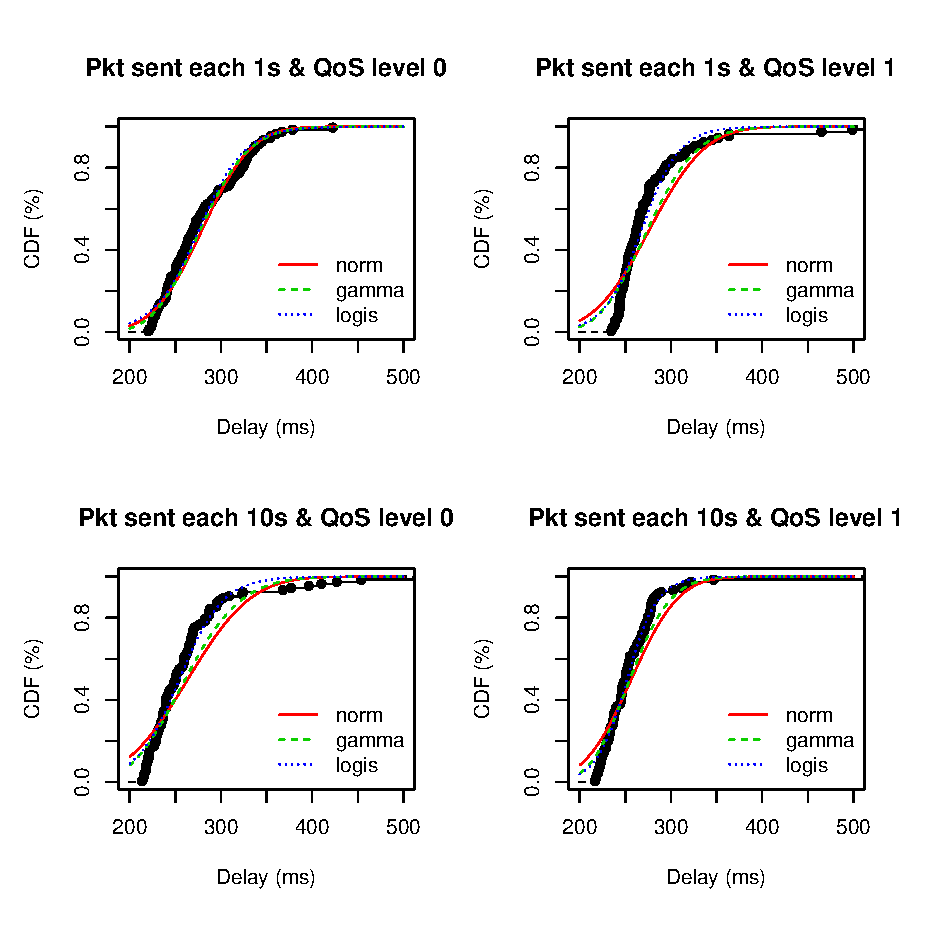
\includegraphics[width=\columnwidth]{distributions_v3.eps}
			\caption{\label{fig:distributions_v3.eps}Distributions}
		\end{figure}
	}{
		\begin{figure}
			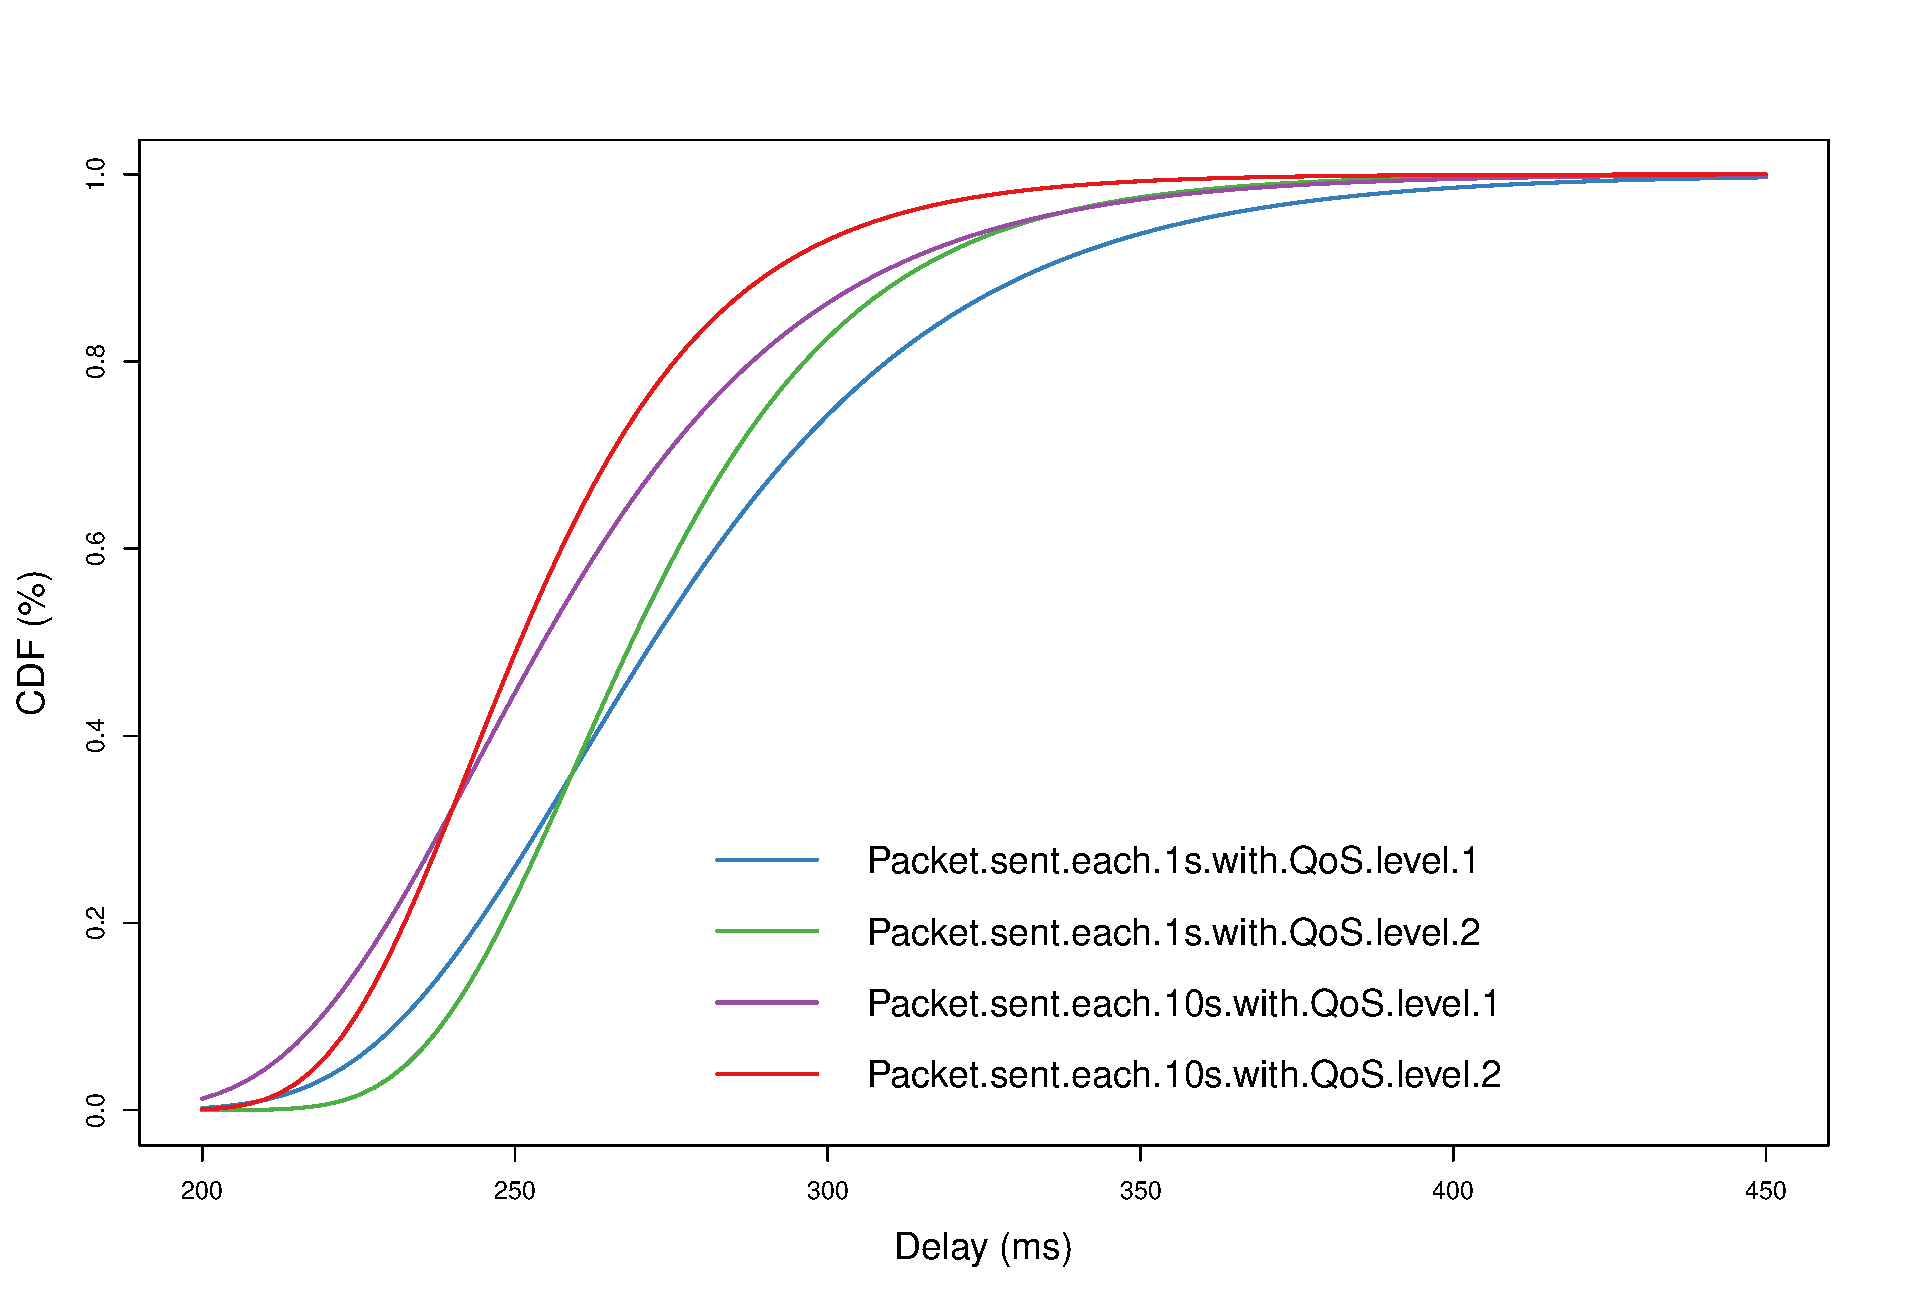
\includegraphics[width=\columnwidth]{res/cdf_v3.eps}
			\caption{\label{fig:cdf_v3.eps}CDF comparison}
		\end{figure}
	}
	
\end{frame}


%	\subsection{Conclusion}
%		\subsection{Conclusion}
\begin{frame}{Conclusion}

	\begin{columns}
		\begin{column}{0.5\textwidth}
%			\newcolumntype{a}{>{\columncolor[gray]{0.8}}c}
			\begin{figure}
				\includegraphics[scale=0.09]{mail.png}
				\caption{\label{fig:g0}Cag.}
			\end{figure}
			\begin{figure}
				\includegraphics[scale=0.09]{mail.png}
				\caption{\label{fig:g1}Cag.}
			\end{figure}
		\end{column}
		\begin{column}{0.5\textwidth}
			\begin{figure}
				\includegraphics[scale=0.09]{mail.png}
				\caption{\label{fig:g2}Cag.}
			\end{figure}
			
			\begin{figure}
				\includegraphics[scale=0.09]{mail.png}
				\caption{\label{fig:g3}Cag.}
			\end{figure}
		\end{column}
	\end{columns}

\end{frame}


%		\begin{frame}[bg]{Challenges}{Conclusion}
	\begin{itemize}
		\item Privacy threats
			\begin{itemize}
				\item Privacy settings
				\item Information propagation
				\item 
			\end{itemize}
		\item Privacy protection
			\begin{itemize}
				\item Privacy settings
				\item I
			\end{itemize}
	\end{itemize}
	\note{L'objectif est de réduire le taux de mortalité}
	\note{L'objectif est de rendre nos route plus sure}
	
	\bey
\end{frame}



%\section{Third contribution}
%	\subsection{Related work}
%		\begin{frame}{State of the art}{Standardization}
	
	\note{
		\begin{itemize}
			\item Contenu:
			\begin{itemize}
				\item Tableau comparatif (articles connexes/avantages et désavantages)
				\item Les limites de l’existant
				\item Notre travaille traite le meme x que les travaux précidants mais utilise y au lieu de z (xy/xz)
			\end{itemize}
			\item Procedure:
			\begin{itemize}
				\item Lecture en largeur
				\begin{itemize}
					\item Lecture de beaucoup de papiers connexes
					\item Comprendre le domaine
					\item Comprendre les travaux existants
					\item Sélection des travaux intéressants
				\end{itemize}
				\item Lecture en profondeur
				\begin{itemize}
					\item Lecture et analyse des travaux sélectionnés
					\item Descendre jusqu’au détail du détail
					\begin{itemize}
						\item Poser toujours la question pourquoi?
						\item Être capable d’implémenter de suite l’approche.
					\end{itemize}
				\end{itemize}
				\item Situer le travail par rapport à l’existant sur la base de La problématique traitée
				\begin{itemize}
					\item Les critiques faites sur l’existant
					\item Les hypothèses du travail courant
					\item Les objectifs initiales du travail
					\item Les résultats théoriques et expérimentales obtenus
				\end{itemize}
			\end{itemize}
			\item Article:
			\begin{itemize}
				\item Est-ce que le problème est toujours intéressant ?
				\item Est-ce qu'on peux traiter le problème d'une autre manière ?
				\item Est-ce que les hypothèses sont réalistes ?
				\item Est-ce que le travail est applicable dans le contexte actuel ?
				\item Est-ce que tous les aspects du problème ont été traités ?
				\item Existe-t-il d’autres manières pour le résoudre ?
			\end{itemize}
		\end{itemize}
	}
\end{frame}


%	\subsection{Contagion process}
%		\subsection{Contagion process}
\begin{frame}{... (step 1)}{Methods}

\Itemize{
	\item S = {SF12, BW125, 4/8, 17 dBm}
	\item Input: 
	\Itemize{
		\item Problem: f(x) = {max($x^{2}$), x \in [0,32]}
		\Itemize{
			\item $x_{1}: 01101_{b}$ 
			\item $x_{2}: 11000_{b}$
			\item $x_{3}: 01000_{b}$
			\item $x_{4}: 10011_{b}$
		}
	}

	\item Method: Genetic algorithm
	\Itemize{
		\item Generate a set of random possible solution
		\item Test each solution and see how good it is (ranking)
		\Enumerate{
			\item Remove some bad solutions
			\item Duplicate some good solutions
			\item Make small changes to some of them (Crossover, Mutation)
		}
	}

	\item Output:
	\Itemize{
			\item $x_{1}$: 01101  (169)  (14.4)
			\item $x_{2}$: 11000  (576)  (49.2)
			\item $x_{3}$: 01000  (64 )  (5.5)
			\item $x_{4}$: 10011  (361)  (30.9)
	}
}
\end{frame}

%\note{
%	\begin{itemize}
%		\item Contenu:
%		\begin{itemize}
%			\item L’approche doit être soigneusement détaillée
%			\item Motiver les étapes, les hypothèses, le contexte
%			\item Dérouler un exemple si nécessaire
%			\item Illustrer par des schémas et figures
%			\item Se concentrer sur les aspects où l’approche apporte une contribution
%			\item Montrer comment on est différent de l’existant
%		\end{itemize}
%		\item Conseils:
%		\begin{itemize}
%			\item Présentation de l'approche utilisée pour résoudre le problème posé: approche(contrainte, parametre du probleme) = solution
%			\begin{itemize}
%				\item Justification du choix de l'approche
%				\item Description générale de l’approche comme une boite noir
%				\begin{itemize}
%					\item Entrées, Sorties, Contraintes, Hypothèses
%				\end{itemize}
%				\item Description détaillée de la solution du problème
%				\begin{itemize}
%					\item Description détaillée des étapes: paramètre -> étape1 -> étape2, ... -> solution
%					\item Modélisation des objets manipulés
%				\end{itemize}
%			\end{itemize}
%			\item Mise en œuvre des hypothèses
%			\item Description de la solution du problème
%		\end{itemize}
%		\item Conseils 2:
%		\begin{itemize}
%			\item Utilisez un exemple pour le dérouler tout au long des étapes de l’approche
%			\item Ne parlez dans ce chapitre que de votre travail, ce qu’ont fait les autres est dans l’état de l’art
%			\item Insistez sur les parties où vous apportez des contributions
%			\item Montrez comment votre travail est différent des autres
%			\item Montrez les modules/algorithmes pris de l’existant, ne réinventez pas la roue.
%			\item le lecteur doit pouvoir reproduire les résultats en appliquant la même approche.
%		\end{itemize}
%	\end{itemize}
%}

\begin{frame}{... (step 2)}{Methods}
	\Itemize{
		\item 
		\item 
	}
\end{frame}

\begin{frame}{... (step 3)}{Methods}
	\Itemize{
		\item 
		\item 
	}
\end{frame}

\begin{frame}{... (step 4)}{Methods}
	\Itemize{
		\item 
		\item 
	}
\end{frame}

\begin{frame}{Results}{Comparison}
	\begin{table}[h!]
	\scriptsize
		\begin{tabulary}{\textwidth}{L|L|L|L|L}
		\  &  &  &  &  \\\hline
		\  &  &  &  &  \\\hline
		\  &  &  &  &  \\\hline
		\  &  &  &  &  \\\hline
		\  &  &  &  &  \\\hline
		\end{tabulary}
	\caption{\label{tab:} }
	\end{table}
\end{frame}


%	\subsection{Experimentation}
%		\subsection{Experimentation}
\begin{frame}{Experimentation}{Experimentation}
	\begin{itemize}
		\item Privacy threats
			\begin{itemize}
				\item Privacy settings
				\item Information propagation
				\item 
			\end{itemize}
		\item Privacy protection
			\begin{itemize}
				\item Privacy settings
				\item I
			\end{itemize}
	\end{itemize}
	
\end{frame}


%	\subsection{Results exploitation}
%		\subsubsection{Context}
%		\subsubsection{Context}
%		\begin{frame}{Results}{Comparison}

	\Columns{0.5}{0.5}{
		\begin{figure}
			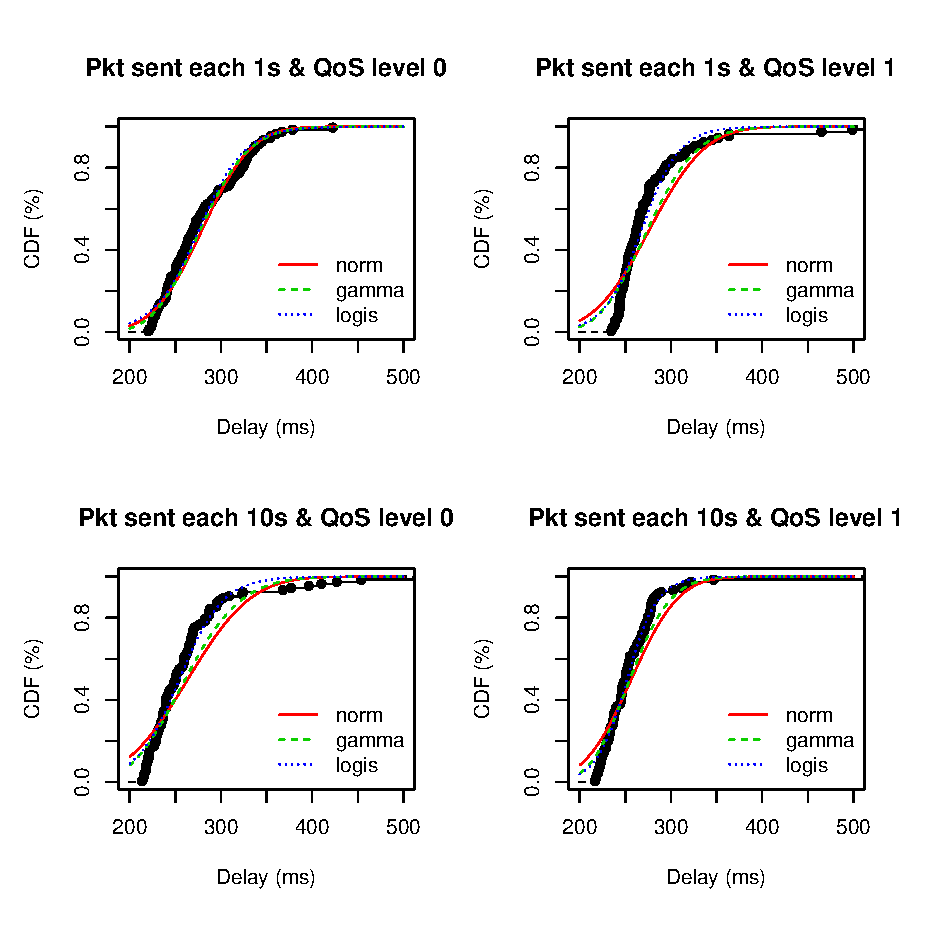
\includegraphics[width=\columnwidth]{distributions_v3.eps}
			\caption{\label{fig:distributions_v3.eps}Distributions}
		\end{figure}
	}{
		\begin{figure}
			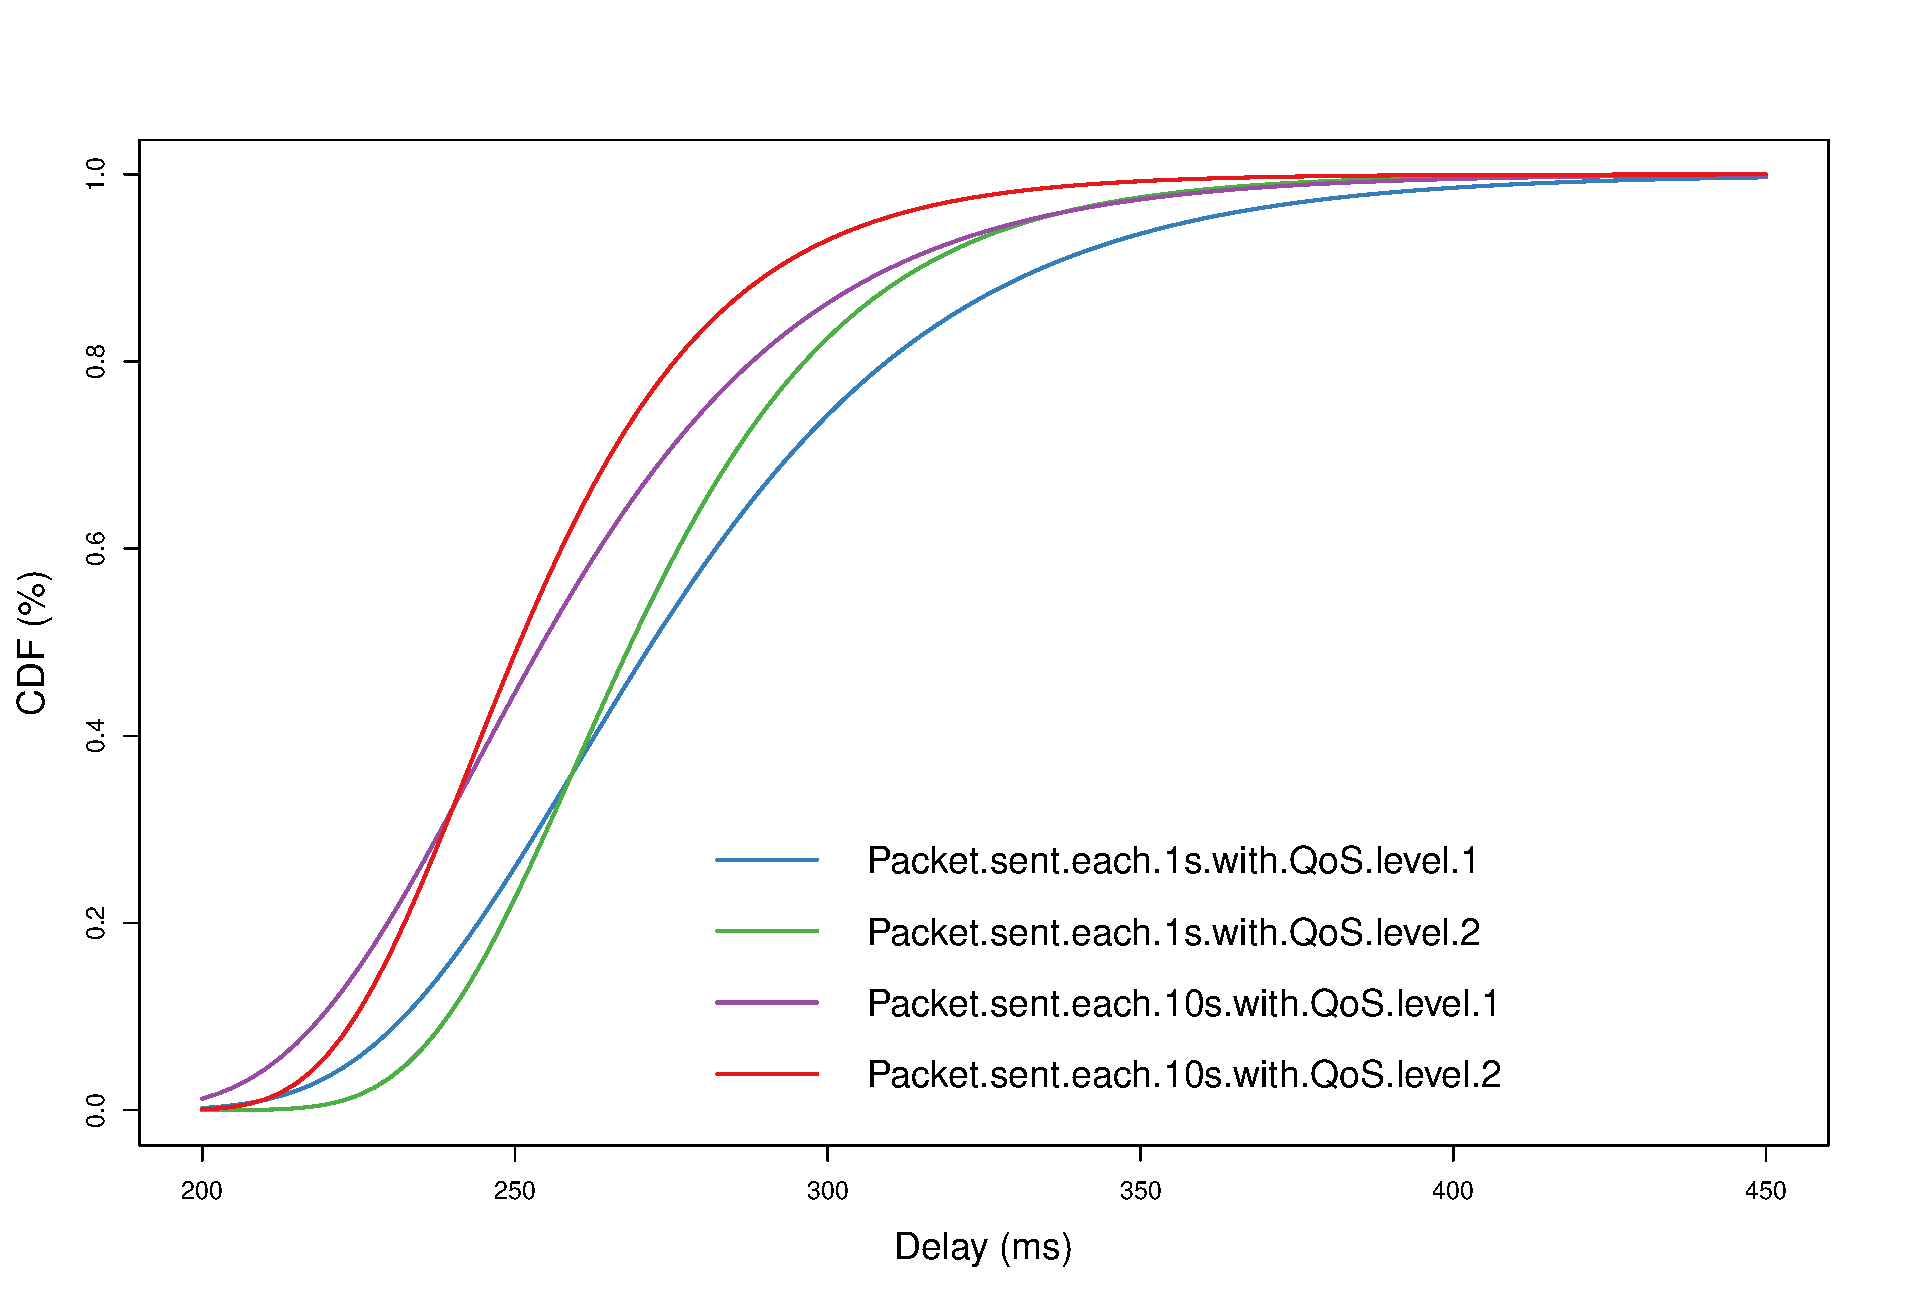
\includegraphics[width=\columnwidth]{res/cdf_v3.eps}
			\caption{\label{fig:cdf_v3.eps}CDF comparison}
		\end{figure}
	}
	
\end{frame}


%	\subsection{Conclusion}
%		\subsection{Conclusion}
\begin{frame}{Conclusion}

	\begin{columns}
		\begin{column}{0.5\textwidth}
%			\newcolumntype{a}{>{\columncolor[gray]{0.8}}c}
			\begin{figure}
				\includegraphics[scale=0.09]{mail.png}
				\caption{\label{fig:g0}Cag.}
			\end{figure}
			\begin{figure}
				\includegraphics[scale=0.09]{mail.png}
				\caption{\label{fig:g1}Cag.}
			\end{figure}
		\end{column}
		\begin{column}{0.5\textwidth}
			\begin{figure}
				\includegraphics[scale=0.09]{mail.png}
				\caption{\label{fig:g2}Cag.}
			\end{figure}
			
			\begin{figure}
				\includegraphics[scale=0.09]{mail.png}
				\caption{\label{fig:g3}Cag.}
			\end{figure}
		\end{column}
	\end{columns}

\end{frame}


%		\begin{frame}[bg]{Challenges}{Conclusion}
	\begin{itemize}
		\item Privacy threats
			\begin{itemize}
				\item Privacy settings
				\item Information propagation
				\item 
			\end{itemize}
		\item Privacy protection
			\begin{itemize}
				\item Privacy settings
				\item I
			\end{itemize}
	\end{itemize}
	\note{L'objectif est de réduire le taux de mortalité}
	\note{L'objectif est de rendre nos route plus sure}
	
	\bey
\end{frame}



\section{Conclusion}
		\begin{frame}{Conclusion}

%\changefontsizes{pt}
\begin{table}[h!]
\begin{center}
	\begin{tabulary}{\textwidth}{L|L|L|L|L}
		\bf{Routing protocol}  & \bf{Control Cost} & \bf{Link Cost} & \bf{Node Cost} \\\hline
		\bf{OSPF/IS-IS}        & \ko               & \ok            & \ko      \\
		\bf{OLSRv2}            & ?                 & \ok            & \ok      \\
%		\bf{TBRPF}             & \ko               & \ok            & ?        \\
		\bf{RIP}               & \ok               & ?              & \ko      \\
%		\bf{AODV}              & \ok               & \ko            & \ko      \\
%		\bf{DYMO}              & \ok               & ?              & ?        \\
		\bf{DSR}               & \ok               & \ko            & \ko      \\
		\bf{RPL}               & \ok               & \ok            & \ok      \\\hline
	\end{tabulary}
	\caption{\label{tab:routingsComaprison} Routing protocols comparison \cite{_rpl2_}}
\end{center}
\end{table}
	
	\begin{table}
	\begin{tabulary}{\textwidth}{C|C|C|C|C|C|C|C}
			\textbf{Application protocol} & RestFull & Transport & Publish/Subscribe & Request/Response & Security & QoS & Header size (Byte)\\\hline
			\textbf{COAP}                 & \ok      & UDP       & \ok               & \ok              & DTLS     & \ok & 4           \\\hline
			\textbf{MQTT}                 & \ko      & TCP       & \ok               & \ko              & SSL      & \ok & 2           \\\hline
			\textbf{MQTT-SN}              & \ko      & TCP       & \ok               & \ko              & SSL      & \ok & 2           \\\hline
			\textbf{XMPP}                 & \ko      & TCP       & \ok               & \ok              & SSL      & \ko & -           \\\hline
			\textbf{AMQP}                 & \ko      & TCP       & \ok               & \ko              & SSL      & \ok & 8           \\\hline
			\textbf{DDS}                  & \ko      & UDP TCP   & \ok               & \ko              & SSL DTLS & \ok & -           \\\hline
			\textbf{HTTP}                 & \ok      & TCP       & \ko               & \ok              & SSL      & \ko & -           \\
		\end{tabulary}
		\caption{\label{tab:protocolsComparison} Application protocols comparison}
	\end{table}
	
	% Commands to include a figure:
	%\begin{figure}
	%\includegraphics[width=\textwidth]{your-figure's-file-name}
	%\caption{\label{fig:your-figure}Caption goes here.}
	%\end{figure}
	
	\note{
		\begin{itemize}
			\item Rappel des objectifs assignés au début
				\item Synthèse de ce qui a été réalisé
				\item Synthèse de ce qui n’a pas été réalisé
				\item Perspectives du travail
				\begin{itemize}
					\item Améliorations, Extensions, Ouvertures
				\end{itemize}
			\item Il ne faut pas s’arrêter
				\begin{itemize}
					\item Effectuer une autocritique
					\item Identifier les aspects qui nécessitent une amélioration
					\item Identifier les éventuelles améliorations du travail
					\begin{itemize}
						\item Nouvelles hypothèses, Nouveau environnement
					\end{itemize}
				\end{itemize}
		\end{itemize}
	}

	\bey
\end{frame}


%		\input{src/2_1_challenges}

%\alltableofcontent

\frameBibliography
\end{document}


%	\subsection{Behavioral}
%	\begin{frame}{Behavioral}{A Behavioural Model for Consumer Reputation \cite{basu_behavioural_2007}}
	
	\begin{columns}
	
		\begin{column}{0.5\textwidth}
				\begin{figure}
					\includegraphics[width=\columnwidth]{res/2_1_1_0.png}
					\caption{\label{fig:g2}Cag.}
				\end{figure}
		\end{column}
		
		\begin{column}{0.5\textwidth}
			\begin{itemize}
				
				%\item[*] good reputation
				
				\item \small{getting better with good behaviour}
					\includegraphics[width=\linewidth]{res/2_1_1_3.png}
					
				\item \small{getting worse with bad behaviour}
					\includegraphics[width=\linewidth]{res/2_1_1_5.png}
					\begin{itemize}
						\item \includegraphics[width=0.6\linewidth]{res/2_1_1_6.png}
					\end{itemize}
					
				%\item[*] bad reputation
					
				\item \small{getting worse with bad behaviour}
					\includegraphics[width=\linewidth]{res/2_1_1_4.png}
					
				\item \small{getting better with good behaviour}
					\includegraphics[width=\linewidth]{res/2_1_1_9.png}
					\begin{itemize}
						\item \includegraphics[width=0.6\linewidth]{res/2_1_1_10.png}
					\end{itemize}
				
				\item \small{positive reputation decaying over time}
					\includegraphics[width=0.7\linewidth]{res/2_1_1_7.png}
					
				\item \small{negative reputation kl increasing over time}
					\includegraphics[width=0.7\linewidth]{res/2_1_1_8.png}
					
			\end{itemize}
		\end{column}
	\end{columns}
	
	\note[item]{Thank the audience for being awake.}
	
\end{frame}

%\begin{frame}{Behavioral}{A Behavioural Model for Consumer Reputation \cite{basu_behavioural_2007}}

%	\begin{columns}
%	
%		\begin{column}{0.6\textwidth}				
%				\begin{figure}
%					\includegraphics[width=\columnwidth]{res/2_1_1_1.png}
%					\caption{\label{fig:g3}Cag.}
%				\end{figure}
%		\end{column}
%		
%		\begin{column}{0.4\textwidth}
%			\begin{itemize}
%			
%				\item \small{good reputation getting better with good behaviour}
%					\includegraphics[width=\linewidth]{res/2_1_1_3.png}
%				
%				\item \small{bad reputation getting worse with bad behaviour}
%					\includegraphics[width=\linewidth]{res/2_1_1_4.png}
%					
%				\item \small{good reputation getting worse with bad behaviour}
%					\includegraphics[width=\linewidth]{res/2_1_1_5.png}
%					\begin{itemize}
%						\item \includegraphics[width=0.6\linewidth]{res/2_1_1_6.png}
%					\end{itemize}
%					
%				\item \small{bad reputation getting better with good behaviour}
%					\includegraphics[width=\linewidth]{res/2_1_1_9.png}
%					\begin{itemize}
%						\item \includegraphics[width=0.6\linewidth]{res/2_1_1_10.png}
%					\end{itemize}
%				
%				\item \small{positive reputation decaying over time}
%					\includegraphics[width=0.7\linewidth]{res/2_1_1_7.png}
%					
%				\item \small{negative reputation increasing over time}
%					\includegraphics[width=0.7\linewidth]{res/2_1_1_8.png}

%			\end{itemize}
%		\end{column}
%	\end{columns}

%\end{frame}


%	\begin{frame}{Behavioral}{Privacy Detective: Detecting Private Information and Collective Privacy Behavior in a Large Social Network \cite{caliskanislam_privacy_2014}}


	\begin{columns}
	
		\begin{column}{0.35\textwidth}
				\begin{center}
					\begin{figure}
						\includegraphics[height=0.15\textheight]{res/2_1_2_0.png}
						\caption{\label{fig:2_1_2_0} User privacy score-1}
					\end{figure}
				
					\begin{figure}
						\includegraphics[height=0.15\textheight]{res/2_1_2_1.png}
						\caption{\label{fig:2_1_2_1} User privacy score-2}
					\end{figure}
				
					\begin{figure}
						\includegraphics[height=0.15\textheight]{res/2_1_2_2.png}
						\caption{\label{fig:2_1_2_2} User privacy score-3}
					\end{figure}
				\end{center}
		\end{column}
		
		\begin{column}{0.65\textwidth}
		
			\begin{itemize}
		
				\item Content based features (Timelines)
				
				\item Amazon mechanical turk annotations (labeling)
					\begin{itemize}
						\item Annotate the publicly available data which is used for calculating the privacy scores.
					\end{itemize}
					
				\item 3-class supervised learning
					\begin{itemize}
				
						\item Timelines are classified with privacy scores by using AdaBoost with Naive Bayes classifier.
				
					\end{itemize}
					
				\item Study the correlation between User’s Privacy Score and:
					\begin{itemize}
					
						\item User’s Friends’ Privacy Score (fig \ref{fig:2_1_2_0}, \ref{fig:2_1_2_1}, \ref{fig:2_1_2_2})
							\begin{itemize}
								\item R value is 0.41, and a two-tailed P value is 0.005.
							\end{itemize}
							
						\item Mentioned (CC) Users’ Privacy Score
							\begin{itemize}
						
								\item R value is 0.37 and a two-tailed P value is 0.01.
								\item Users prefer to follow users that have similar privacy revealing habits.
						
							\end{itemize}
							
						\item Number of Friends
							\begin{itemize}
						
								\item There is no statistically significant correlation between a user’s privacy score and the number of friends.
						
							\end{itemize}
							
					\end{itemize}
		
			\end{itemize}
		
		\end{column}
	\end{columns}

\end{frame}


%	\begin{frame}{Behavioral}{Detecting and resolving privacy conflicts for collaborative data sharing in online social networks \cite{hu_detecting_2011}}


%	\mbox{}
	\hfill
	\raisebox{-\height}[0pt][0pt]{\includegraphics[width=.4\linewidth]{res/2_1_3_5.png}}
%	\vspace*{-\baselineskip}

	\begin{itemize}

		\item Input

			\begin{itemize}

				\item Number of privacy conflicts $ controllers_{ut} (i)$
					\begin{itemize}
						\item number of the untrusting controllers 
					\end{itemize}
			
				\item General privacy concern of an untrusting controller $pc_{j}$
				\item Sensitivity of the data item $sl_{j}$
				\item Visibility of the data item
				\item Trust of an accessor $tl_{k}$ (MTA)

			\end{itemize}
	
		\item[$\bullet$]  Measuring Privacy Risk:
	
			\begin{itemize}
				\item[]	\includegraphics[scale=0.07]{res/2_1_3_0.png}
				\item[]	\includegraphics[scale=0.07]{res/2_1_3_1.png}
			\end{itemize}
	
	
		\item[$\bullet$]	Measuring Sharing Loss:

			\begin{itemize}
				\item[]	\includegraphics[scale=0.1]{res/2_1_3_3.png}
			\end{itemize}

		\item[$\bullet$]	Privacy Conflict Resolution on the Tradeoff between Privacy Protection and Data Sharing:

			\begin{itemize}
				\item[]	\includegraphics[scale=0.08]{res/2_1_3_4.png}
			\end{itemize}
	

	\end{itemize}
	
\end{frame}


%	\subsubsection{Aghiles}
%	\begin{frame}{Trust Model}{Computational Trust Model for Repeated Trust Games \cite{dang_computational_2016}}

		\begin{columns}[T]
			\begin{column}{0.4\textwidth}
				\begin{flushleft}
				
					\begin{itemize}
						\item[] \includegraphics[width=\columnwidth]{res/2_1_4_0.png}
						\item[] \includegraphics[width=\columnwidth]{res/2_1_4_1.png}
						\item[] \includegraphics[width=\columnwidth]{res/2_1_4_2.png}
						\item[] \includegraphics[width=\columnwidth]{res/2_1_4_3.png}
						\item[] \includegraphics[width=0.8\columnwidth]{res/2_1_4_4.png}
					\end{itemize}
				
				\end{flushleft}
			\end{column}
			
			\begin{column}{0.4\textwidth}
				\begin{center}
				
					\begin{itemize}
						\item[] \includegraphics[width=\columnwidth]{res/2_1_4_5.png}
						\item[] \includegraphics[width=\columnwidth]{res/2_1_4_6.png}
					\end{itemize}
					
				\end{center}
			\end{column}
		\end{columns}
		
\end{frame}


%	\begin{frame}{Behavioral}{Styx: Privacy risk communication for the Android smartphone platform based on apps' data-access behavior patterns \cite{bal_styx_2015}}

	\begin{columns}
		\begin{column}{0.5\textwidth}
			\begin{center}
			
				\begin{figure}
					\includegraphics[width=\columnwidth]{res/2_1_5_0.png}
					\caption{\label{fig:2_1_5_0}Cag.}
				\end{figure}
				
			\end{center}
		\end{column}
		
		\begin{column}{0.5\textwidth}
		
			\begin{itemize}
				\item 
				
				\item 
					\begin{itemize}
						\item 
						\item 
					\end{itemize}
				
				\item 
			\end{itemize}
			
		\end{column}
	\end{columns}
	

\end{frame}


%	\begin{frame}{Behavioral}{Exploring nuances of user privacy preferences on a platform for political participation \cite{kaskina_exploring_2017}}
		
				\begin{figure}
					\includegraphics[width=0.7\columnwidth]{res/2_1_6_0.png}
					\caption{\label{fig:2_1_6_0}hh}

					\includegraphics[width=0.7\columnwidth]{res/2_1_6_1.png}
					\caption{\label{fig:2_1_6_1}hh}
				\end{figure}
		
\end{frame}


%	\subsubsection{Boumerdes}
%	\begin{frame}{Behavioral}{Prometheus: User-controlled P2P Social Data Management for Socially-aware Applications \cite{kourtellis_prometheus_2010}}

	\begin{columns}
		\begin{column}{0.5\textwidth}
			\begin{center}
			
				\begin{figure}
					\includegraphics[width=\columnwidth]{res/2_1_7_0.png}
					\caption{\label{fig:2_1_7_0}Geo-social Graph Representation}
					
					\includegraphics[width=0.5\columnwidth]{res/2_1_7_1.png}
					\caption{\label{fig:2_1_7_1}Example of an access control policy}
				\end{figure}
				
			\end{center}
		\end{column}
		
		\begin{column}{0.5\textwidth}
		
			\begin{itemize}
				\item Trusted Peer Group Management
				
				\item 
					\begin{itemize}
						\item 
						\item 
					\end{itemize}
				
				\item 
			\end{itemize}
			
		\end{column}
	\end{columns}
	

\end{frame}


%%	\begin{frame}{Behavioral}{On Multi-Dimensional Privacy in Context-Aware Mobile Networks \cite{bilogrevic_multidimensional_2014}}

	\begin{columns}
		\begin{column}{0.5\textwidth}
			\begin{center}
			
				\begin{figure}
					\includegraphics[width=\columnwidth]{res/2_1_8_0.png}
					\caption{\label{fig:2_1_8_0}hghg}
				\end{figure}
				
			\end{center}
		\end{column}
		
		\begin{column}{0.5\textwidth}
		
			\begin{itemize}
				\item 
				
				\item 
					\begin{itemize}
						\item 
						\item 
					\end{itemize}
				
				\item 
			\end{itemize}
			
		\end{column}
	\end{columns}
	

\end{frame}


%	\begin{frame}{Behavioral}{Computing Privacy Risk and Trustworthiness of Users in {SNSs} \cite{pandey_computing_2015}}

	\begin{columns}
		\begin{column}{0.7\textwidth}
			\begin{center}
			
				\begin{figure}
					\includegraphics[width=\columnwidth]{res/2_1_9_0.png}
					\caption{\label{fig:2_1_9_0} Relationship between user’s trustworthiness and privacy risk}
				\end{figure}
				
			\end{center}
		\end{column}
		
		\begin{column}{0.3\textwidth}
		
			\begin{itemize}
				\item 
				
				\item 
					\begin{itemize}
						\item 
						\item 
					\end{itemize}
				
				\item 
			\end{itemize}
			
		\end{column}
	\end{columns}
	

\end{frame}


%%	\begin{frame}{Behavioral}{Understanding Site-Based Inference Potential for Identifying Hidden Attributes \cite{moore_understanding_2013}}

	\begin{columns}
		\begin{column}{0.5\textwidth}
			\begin{center}
			
				\begin{figure}
					\includegraphics[width=\columnwidth]{res/2_1_10_0.png}
					\caption{\label{fig:2_1_10_0}Attribute inference methodology.}
				\end{figure}
				
			\end{center}
		\end{column}
		
		\begin{column}{0.5\textwidth}
		
			\begin{itemize}
				\item 
				
				\item 
					\begin{itemize}
						\item 
						\item 
					\end{itemize}
				
				\item 
			\end{itemize}
			
		\end{column}
	\end{columns}
	

\end{frame}

\begin{frame}[noframenumbering]{Behavioral}{Understanding Site-Based Inference Potential for Identifying Hidden Attributes \cite{moore_understanding_2013}}
			
				\begin{figure}
					\includegraphics[width=\columnwidth]{res/2_1_10_1.png}
					\caption{\label{fig:2_1_10_1}LDA inference engine.}
				\end{figure}
	
\end{frame}


%	
%	\subsection{Social}
%	\begin{frame}{Social}{A Study of Online Social Network Privacy Via the {TAPE} Framework \cite{yongbozeng_study_2015}}

	\begin{columns}
		\begin{column}{0.35\textwidth}
			\begin{center}
			
				\begin{figure}
					\includegraphics[width=\columnwidth]{res/2_2_1_0.png}
					\caption{\label{fig:2_2_1_0}Cag.}
				\end{figure}
				
				\begin{figure}
					\includegraphics[width=\columnwidth]{res/2_2_1_1.png}
					\caption{\label{fig:2_2_1_1}Cag.}
				\end{figure}
				
			\end{center}
		\end{column}
		
		\begin{column}{0.65\textwidth}
		
			\begin{itemize}
				\item Node Information Spreading (NISP)
					\begin{itemize}
						\item How likely a friend will spread other's PI ? 
					\end{itemize}
					
				\item Methods
					\begin{itemize}
						\item TAPE: The friend with the largest Birnbaum's measure is blocked.
							\begin{itemize}
								\item Evaluate the sensitivity of a friend link
							\end{itemize}
					

						\item Friend Degree: The friend that has the largest degree is blocked.
							\begin{itemize}
								\item Evaluate the importance of a friend link
							\end{itemize}
					

						\item V-Index: The friend that has the largest V-Index is blocked.
							\begin{itemize}
								\item Evaluate privacy setting of a friend ...
							\end{itemize}
					

						\item Random: Random friends are blocked.
							\begin{itemize}
								\item Privacy risk decrease as undesirable destination (NISP) blocked
							\end{itemize}
					\end{itemize}
					
				\item[-] Privacy risk decrease as undesirable destination (NISP) blocked
					
					\bigskip
					
				\item Link Information Spreading (LISP)
					\begin{itemize}
						\item How likely a friend will be in the path of PI diffusion
					\end{itemize}
					

				\item[-] Privacy risk increase as LISP increase and distance decrease.

			\end{itemize}
			
		\end{column}
	\end{columns}
	

\end{frame}


%	\begin{frame}{Social}{Algorithm to trade off between utility and privacy cost of online social search \cite{li_algorithm_2016}}

	\begin{columns}
		\begin{column}{0.34\textwidth}
			\begin{center}
			
				\begin{figure}
					\includegraphics[width=\columnwidth]{res/2_2_2_0.png}
					\caption{\label{fig:2_2_2_0}Cag.}
				\end{figure}
				
				\begin{figure}
					\includegraphics[width=\columnwidth]{res/2_2_2_1.png}
					\caption{\label{fig:2_2_2_1}Cag.}
				\end{figure}
				
			\end{center}
		\end{column}
		
		\begin{column}{0.66\textwidth}
		
			\begin{itemize}
				\item Input:
					\begin{itemize}
						\item p:  Probability of influence from u to v.
						\item dv:  Degree of the node v.
						\item sv:  Number of neighbors of v who are seeds.
						\item tv: Number of neighbors of v who are seeds and experts
					\end{itemize}

				\item Method:
					\begin{itemize}
						\item Utility Degree Discount Algorithm:
							\begin{itemize}
								\item If (expert) \hspace{3mm} $d_{dv}$ = $(1 - p)^{sv}$ [1 + (dv - tv)]
								\item Else \hspace{9mm} $d_{dv}$ = $(1 - p)^{sv}$ \hspace{4mm} (dv - tv)
							\end{itemize}
							
						\item Utility Privacy Cost Ratio Discount Algorithm:
							\begin{itemize}
								\item If (expert) \hspace{3mm} $d_{dv}$ = $(1 - p)^{sv}$ [1 + (dv - tv)] / (dv - sv)
								\item Else \hspace{9mm} $d_{dv}$ = $(1 - p)^{sv}$ \hspace{5mm} (dv - tv) / (dv - sv)
							\end{itemize}
							
					\end{itemize}
					
				\item Output:
					\begin{itemize}
						\item Privacy: Number of seeds activated (FP)
						\item Utility: Number of expert activated (TP)
					\end{itemize}
					
				\item Note: (1 - p)sv · [1 + (dv - tv) . p] Expected number of additional nodes influenced by v

			\end{itemize}
		\end{column}
	\end{columns}

\end{frame}


%	\begin{frame}{Social}{Privacy scoring of social network users as a service \cite{vidyalakshmi_privacy_2015}}

	\begin{columns}
		\begin{column}{0.39\textwidth}
			\begin{center}
			
				\begin{figure}
					\includegraphics[width=\columnwidth]{res/2_2_3_0.png}
					\caption{\label{fig:2_2_3_0}\tiny{Experiment results with varying l0 and h0}}
					
					\includegraphics[width=\columnwidth]{res/2_2_3_1.png}
					\caption{\label{fig:2_2_3_1} \tiny{Naive vs Proposed privacy scoring}}
				\end{figure}
				
			\end{center}
		\end{column}
		
		\begin{column}{0.61\textwidth}
		
			\begin{itemize}

				\item Input
					\begin{itemize}
					
						\item l0 [0, 1] : Disposition to privacy:
							\begin{itemize}
								\item Attitude of an user towards privacy of his information.
								\item l0 = 0,1 :  Lax privacy orientation 
							\end{itemize}
							
						\item h0 [0, 1] : Disposition to communication:
							\begin{itemize}
								\item Attitude of an user towards communication online.
								\item h0 = 0.1 :  User who is very communication oriented
							\end{itemize}
						
						\item Friend Attitude Calculator (FACT):
							\begin{itemize}
								\item Pn: The friends position in the sorted trust list.
								\item Cn: The percentage of total communication.
								\item tx: Total number of friends.
							
								\item[] \includegraphics[width=0.7\linewidth]{res/2_2_3_2.png}
							\end{itemize}
					\end{itemize}
							
				\item Method: (cubic bezier curve)
					\begin{itemize}
						\item[] \includegraphics[width=0.8\linewidth]{res/2_2_3_3.png}
					\end{itemize}
					

				\item Output:
					\begin{itemize}
						\item Privacy score: $PS_{l0,h0}$ (xn)
					\end{itemize}
					
			\end{itemize}
			
		\end{column}
	\end{columns}
	
\end{frame}

\begin{frame}[noframenumbering]{Social}{Privacy scoring of social network users as a service \cite{vidyalakshmi_privacy_2015}}

	\begin{columns}
		\begin{column}{0.32\textwidth}
			\begin{center}
			
				\begin{figure}
					\includegraphics[width=\columnwidth]{res/2_2_3_4.png}
					\caption{\label{fig:2_2_3_5}\tiny{Experiment results with varying l0 and h0}}
					
					\includegraphics[width=\columnwidth]{res/2_2_3_5.png}
					\caption{\label{fig:2_2_3_6} \tiny{Naive vs Proposed privacy scoring}}
				\end{figure}
				
			\end{center}
		\end{column}
		
		\begin{column}{0.61\textwidth}
		
			\begin{itemize}

				\item Input
					\begin{itemize}
					
						\item l0 [0, 1] : Disposition to privacy:
							\begin{itemize}
								\item Attitude of an user towards privacy of his information.
								\item l0 = 0,1 :  Lax privacy orientation 
							\end{itemize}
							
						\item h0 [0, 1] : Disposition to communication:
							\begin{itemize}
								\item Attitude of an user towards communication online.
								\item h0 = 0.1 :  User who is very communication oriented
							\end{itemize}
						
						\item Friend Attitude Calculator (FACT):
							\begin{itemize}
								\item Pn: The friends position in the sorted trust list.
								\item Cn: The percentage of total communication.
								\item tx: Total number of friends.
							
								\item[] \includegraphics[width=0.7\linewidth]{res/2_2_3_2.png}
							\end{itemize}
					\end{itemize}
							
				\item Method: (cubic bezier curve)
					\begin{itemize}
						\item[] \includegraphics[width=0.8\linewidth]{res/2_2_3_3.png}
					\end{itemize}
					

				\item Output:
					\begin{itemize}
						\item Privacy score: $PS_{l0,h0}$ (xn)
					\end{itemize}
					
			\end{itemize}
			
		\end{column}
	\end{columns}
	
\end{frame}


%	\begin{frame}{Social}{Privometer: Privacy protection in social networks \cite{talukder_privometer_2010}}

	\begin{columns}
		\begin{column}{0.5\textwidth}
			\begin{center}
				
				\begin{figure}
					\includegraphics[width=0.45\columnwidth]{res/2_2_4_2.png}
					\caption{\label{fig:2_2_4_3} Information Visibility in User Profile}

					\includegraphics[width=0.65\columnwidth]{res/2_2_4_1.png}
					\caption{\label{fig:2_2_4_1} Adversary Model with Malicious Application}
				\end{figure}
				
			\end{center}
		\end{column}
		
		\begin{column}{0.5\textwidth}
			
			\includegraphics[width=\columnwidth]{res/2_2_4_3.png}
			
			\begin{figure}
				\includegraphics[width=\columnwidth]{res/2_2_4_0.png}
				\caption{\label{fig:2_2_4_0} Privometer}
			\end{figure}
			
		\end{column}
	\end{columns}
	

\end{frame}


%	\begin{frame}{Social}{Privacy impact assessment for online social networks \cite{wang_privacy_2015}}

	\begin{columns}
		\begin{column}{0.5\textwidth}
			\begin{center}
			
				\begin{figure}
					\includegraphics[width=\columnwidth]{res/2_2_5_0.png}
					\caption{\label{fig:2_2_5_0} Data loss and Privacy Impact}
				\end{figure}
				
			\end{center}
		\end{column}
		
		\begin{column}{0.5\textwidth}
			
			\begin{itemize}
			
				\item Direct Data Loss (Access control models)
					\begin{itemize}
						\item I-BAC: Individual-Based Access Control
						\item A-BAC: Authority-Based Access Control
						
						\item T-BAC: Team-Based Access Control
							\begin{itemize}
								\item R-BAC: Role-Based Access Control
								\item Or-BAC: Organization-Based Access Control
								\item Re-BAC: Relationship-Based Access Control

							\end{itemize}
					\end{itemize}
					
				\item Indirect Data Loss
					\begin{itemize}
						\item Inference, aggregation, and de-anonymization.
					\end{itemize}
					
				\item Potential Data Loss
					\begin{itemize}
						\item Social engineering, phishing.
					\end{itemize}
					
			\end{itemize}
			
		\end{column}
	\end{columns}
	
\end{frame}


%	\begin{frame}{Social}{Privacy-triggered communications in pervasive social networks \cite{jadliwala_privacytriggered_2011}}

	\begin{columns}
		\begin{column}{0.4\textwidth}
			\begin{center}
			
				\begin{figure}
					\includegraphics[width=\columnwidth]{res/2_2_6_0.png}
					\caption{\label{fig:2_2_6_0} Prototype}
				\end{figure}
				
			\end{center}
		\end{column}
		
		\begin{column}{0.6\textwidth}
		
			\begin{itemize}
			
				\item Input:
					\begin{itemize}
						\item s: Device privacy (state)
						\item b: Message privacy (action)
						\item R: Reward
						\item u: Stationary policy 
					\end{itemize}
					
				\item Method:
					\begin{itemize}
						\item $P_{ij}$ is the probability to transition from state si to sj at time t
							\begin{itemize}
								\item[] \includegraphics[width=0.5\columnwidth]{res/2_2_6_1.png}
							\end{itemize}
							
						
						\item Random variable
							\begin{itemize}
								\item[] \includegraphics[width=0.5\columnwidth]{res/2_2_6_2.png}
								\item X: device state, delta: action chosen at time period t
							\end{itemize}
							
						\item Bellman’s equation
							\begin{itemize}
								\item[] \includegraphics[width=0.7\columnwidth]{res/2_2_6_3.png}
							\end{itemize}
							
					\end{itemize}
					
				\item Output:
					\begin{itemize}
						\item Recommendation to send a message 
					\end{itemize}
					
			\end{itemize}
		\end{column}
	\end{columns}
	

\end{frame}


%	\begin{frame}{Social}{A Framework for Computing the Privacy Scores of Users in Online Social Networks \cite{liu_framework_2010}}

	\begin{columns}
		\begin{column}{0.7\textwidth}
			\begin{center}
			
				\begin{table}
					\begin{tabular}{c|c|c|c|c|c}
															&								&		Sensitivity	&	$\beta_{1}$	&		...			&	$\beta_{n}$	\\\hline
						 	Privacy					&		Attitude		&	User/item			&	item 1			&			...		&	item n			\\\hline
							$P_{1}$					&$\theta_{1}$		&		User 1			&		...				&		...			&			...			\\\hline
								...						&			...				&			...				&		...				&		R(i,j)	&			...			\\\hline
							$P_{N}$					&$\theta_{N}$		&		User N			&		...				&		...			&			...			
					\end{tabular}
					\caption{\label{tab:Table} An example table.}
				\end{table}
				
				
				\includegraphics[width=0.6\columnwidth]{res/2_2_7_1.png}
				
			\end{center}
		\end{column}
		
		\begin{column}{0.2\textwidth}
		
			\begin{center}
				\includegraphics[width=\columnwidth]{res/2_2_7_0.png}
			\end{center}
			
		\end{column}
	\end{columns}
			

\end{frame}


%	\begin{frame}{Social}{Predicting friendship levels in online social networks \cite{ahmad_predicting_2010}}

	\begin{columns}
		\begin{column}{0.4\textwidth}
			\begin{center}
			
				\begin{figure}
					\includegraphics[width=\columnwidth]{res/2_2_8_0.png}
					\caption{\label{fig:2_2_8_0}Levels of OSN}
					
					\includegraphics[width=\columnwidth]{res/2_2_8_1.png}
					\caption{\label{fig:2_2_8_1}Levels of OSN}
				\end{figure}
				
			\end{center}
		\end{column}
		
		\begin{column}{0.6\textwidth}
		
				\begin{figure}
					\includegraphics[width=\columnwidth]{res/2_2_8_2.png}
					\caption{\label{fig:2_2_8_2}Levels of OSN}
				\end{figure}
			
		\end{column}
	\end{columns}
	
\end{frame}


%%	\begin{frame}{Social}{Leveraging Email based Social Networks to Prevent Spam: Framework, System Design and Evaluation \cite{hameed_leveraging_2012}}

\end{frame}


%	\begin{frame}{Social}{Risks of Friendships on Social Networks \cite{akcora_risks_2012}}

	\begin{columns}
		\begin{column}{0.4\textwidth}
			\begin{center}
			
				\begin{figure}
					\includegraphics[width=\columnwidth]{res/2_2_10_0.png}
					\caption{\label{fig:2_2_10_0}H}
				\end{figure}
				
			\end{center}
		\end{column}
		
		\begin{column}{0.6\textwidth}
		
			\begin{itemize}
			
				\item Social Frequency Matrix for friends: N x F x n
					\begin{itemize}
						\item N: user, F: friends, n: friends features
					\end{itemize}
					

				\item Transformation:
					\begin{itemize}
						\item Transform friends features into numerical form
						\item Hometown = Rome: Hometown = 15/100 
					\end{itemize}
					
				\item Baseline Estimation:
					\begin{itemize}
						\item Logistic regression analysis of features.
						\item Ex: \%0.9 very risky, \%0.09 risky and \%0.01 not risky. 
					
					\end{itemize}
				\item Learning Friend Impacts: 
					\begin{itemize}
						\item Past Labeling Parameter
							\begin{itemize}
								\item PS: Profile similarity
							\end{itemize}
							
						\item Friend Impact Parameter
							\begin{itemize}
								\item Single Impact for the Friend Cluster
								\item Multiple Impact for the Friend Cluster
							\end{itemize}
							
					\end{itemize}
			\end{itemize}
			
		\end{column}
	\end{columns}
	

\end{frame}


%	\begin{frame}{Social}{unfriendly: Multi-party privacy risks in social networks \cite{thomas_unfriendly_2010}}

			
	\begin{figure}
		\includegraphics[width=0.8\columnwidth]{res/2_2_11_0.png}
		\caption{\label{fig:2_2_11_0}hghg}
	\end{figure}
				
	\begin{itemize}
		\item 
		
		\item 
			\begin{itemize}
				\item 
				\item 
			\end{itemize}
		
		\item 
	\end{itemize}
	
\end{frame}

%%	\begin{frame}{Social}{Mobile social networking: reconnect virtual community with physical space \cite{zhang_mobile_2013}}

	\begin{columns}
		\begin{column}{0.7\textwidth}
			\begin{center}
			
				\begin{figure}
					\includegraphics[width=\columnwidth]{res/2_2_12_0.png}
					\caption{\label{fig:2_2_12_0}Relationship of MSN with IoT, OSN and mobile computing}
				\end{figure}
				
			\end{center}
		\end{column}
		
		\begin{column}{0.3\textwidth}
		
			\begin{itemize}
				\item 
				
				\item 
					\begin{itemize}
						\item 
						\item 
					\end{itemize}
				
				\item 
			\end{itemize}
			
		\end{column}
	\end{columns}
	

\end{frame}



%	
%	\subsection{Technical}
%	\begin{frame}{Social}{{SocialFilter}: Collaborative Spam Mitigation Using Social Networks \cite{yang_socialfilter_2009}}

	\begin{columns}
		\begin{column}{0.55\textwidth}
			\begin{center}
			
				\begin{figure}
					\includegraphics[width=0.5\columnwidth]{res/2_3_1_0.png}
					\caption{\label{fig:2_3_1_0}Cag.}
				\end{figure}
				
				\begin{figure}
					\includegraphics[width=0.9\columnwidth]{res/2_3_1_1.png}
					\caption{\label{fig:2_3_1_1}Cag.}
				\end{figure}
				
			\end{center}
		\end{column}
		
		\begin{column}{0.45\textwidth}
		
			\begin{enumerate}
			
				\item Confidence: (trust)
					\begin{itemize}
						\item c1 (IP) = 50  and c2 (IP) = 100%
					\end{itemize}
					

				\item The reporter trust $rt_{ij}$
					\begin{itemize}
						\item \includegraphics[width=0.5\columnwidth]{res/2_3_1_2.png}
							\begin{itemize}
								\item P: set of path between i and j.
								\item $d_{uv}$: trust degree between u and v.
							\end{itemize}
						\item $rt_{31}$ = 0.4 and  $rt_{32}$ = 0.648
					\end{itemize}
					
				\item Identity uniqueness
					\begin{itemize}
						\item $id_{1}$ = 0.9 and $id_{2}$ = 0.8
					\end{itemize}
					
			\end{enumerate}
		\end{column}
	\end{columns}

\end{frame}


%	\begin{frame}{Technical}{Privacy-Aware Web Service Composition and Ranking \cite{costante_privacyaware_2013}}

	\begin{columns}
		\begin{column}{0.5\textwidth}
			\begin{center}
			
				\begin{figure}
					\includegraphics[width=\columnwidth]{res/2_3_2_0.png}
					\caption{\label{fig:2_1_5_0} Privacy-Aware Architecture}
				\end{figure}
				
				\begin{figure}
					\includegraphics[width=\columnwidth]{res/2_3_2_1.png}
					\caption{\label{fig:2_1_5_1} Bob’s privacy preferences}
				\end{figure}
				
			\end{center}
		\end{column}
		
		\begin{column}{0.5\textwidth}
		
			\begin{itemize}
				\item 
				
				\item 
					\begin{itemize}
						\item 
						\item 
					\end{itemize}
				
				\item 
			\end{itemize}
			
		\end{column}
	\end{columns}
	

\end{frame}


%	\begin{frame}{Technical}{Ostra: Leveraging trust to thwart unwanted communication \cite{mislove_ostra_2008}}

\end{frame}


%	\begin{frame}{Technical}{On the Design of Socially-Aware Distributed Systems \cite{kourtellis_design_2012}}


	\begin{columns}
		\begin{column}{0.5\textwidth}
			\begin{center}
			
				\begin{figure}
					\includegraphics[width=\columnwidth]{res/2_3_4_0.png}
					\caption{\label{fig:2_3_4_0} different system levels}
				\end{figure}
				
			\end{center}
		\end{column}
		
		\begin{column}{0.5\textwidth}
		
			\begin{itemize}
				\item 
				
				\item 
					\begin{itemize}
						\item 
						\item 
					\end{itemize}
				
				\item 
			\end{itemize}
			
		\end{column}
	\end{columns}
	

\end{frame}


%%	\begin{frame}{Technical}{I know what you did last summer: risks of location data leakage in mobile and social computing \cite{jedrzejczyk_i_2009}}

	\begin{columns}
		\begin{column}{0.7\textwidth}
			\begin{center}
			
				\begin{figure}
					\includegraphics[width=\columnwidth]{res/2_3_5_0.png}
					\caption{\label{fig:2_3_5_0}Relation between usability, privacy and security}
				\end{figure}
				
			\end{center}
		\end{column}
		
		\begin{column}{0.3\textwidth}
		
			\begin{itemize}
				\item 
				
				\item 
					\begin{itemize}
						\item 
						\item 
					\end{itemize}
				
				\item 
			\end{itemize}
			
		\end{column}
	\end{columns}
	

\end{frame}


%	\begin{frame}{Technical}{A privacy self-assessment framework for online social networks \cite{pensa_privacy_2017}}

	\begin{columns}
		\begin{column}{0.4\textwidth}
			\begin{center}
			
				\begin{figure}
					\includegraphics[width=\columnwidth]{res/2_3_6_0.png}
					\caption{\label{fig:2_3_6_0}Privacy scores}
					
					\includegraphics[width=\columnwidth]{res/2_3_6_1.png}
					\caption{\label{fig:2_3_6_1}Privacy scores (AUC)}
				\end{figure}
				
			\end{center}
		\end{column}
		
		\begin{column}{0.6\textwidth}
		
			\begin{itemize}
				\item 
				
				\item 
					\begin{itemize}
						\item 
						\item 
					\end{itemize}
				
				\item 
			\end{itemize}
			
		\end{column}
	\end{columns}
	

\end{frame}


%%	\begin{frame}{Technical}{Filtering Spam with Behavioral Blacklisting \cite{ramachandran_filtering_2007}}

	\begin{columns}
		\begin{column}{0.5\textwidth}
			\begin{center}
			
				\begin{figure}
					\includegraphics[width=\columnwidth]{res/2_3_7_0.png}
					\caption{\label{fig:2_3_7_0}hghgg}
				\end{figure}
				
			\end{center}
		\end{column}
		
		\begin{column}{0.5\textwidth}
		
			\begin{itemize}
				\item 
				
				\item 
					\begin{itemize}
						\item 
						\item 
					\end{itemize}
				
				\item 
			\end{itemize}
			
		\end{column}
	\end{columns}
	

\end{frame}


%%	\begin{frame}{Technical}{ProMail: Using Progressive Email Social Network for Spam Detection \cite{tseng_promail_2007}}

	\begin{columns}
		\begin{column}{0.7\textwidth}
			\begin{center}
			
				\begin{figure}
					\includegraphics[width=\columnwidth]{res/2_3_8_0.png}
					\caption{\label{fig:2_3_8_0}hghg}
				\end{figure}
				
			\end{center}
		\end{column}
		
		\begin{column}{0.3\textwidth}
		
			\begin{itemize}
				\item 
				
				\item 
					\begin{itemize}
						\item 
						\item 
					\end{itemize}
				
				\item 
			\end{itemize}
			
		\end{column}
	\end{columns}
	

\end{frame}


%	\begin{frame}{Technical}{A privacy awareness system for facebook users \cite{helou_privacy_2012}}

	\begin{columns}
		\begin{column}{0.8\textwidth}
			\begin{center}
			
				\begin{figure}
					\includegraphics[width=\columnwidth]{res/2_3_9_0.png}
					\caption{\label{fig:2_3_9_0}}
					
					\includegraphics[width=\columnwidth]{res/2_3_9_1.png}
					\caption{\label{fig:2_3_9_1}}
				\end{figure}
				
			\end{center}
		\end{column}
		
		\begin{column}{0.2\textwidth}
		
			\begin{itemize}
				\item 
				
				\item 
					\begin{itemize}
						\item 
						\item 
					\end{itemize}
				
				\item 
			\end{itemize}
			
		\end{column}
	\end{columns}
	

\end{frame}


%	\begin{frame}{Technical}{Identifying hidden social circles for advanced privacy configuration \cite{squicciarini_identifying_2014}}

	\begin{columns}
		\begin{column}{0.5\textwidth}
			\begin{center}
			
				\begin{figure}
					\includegraphics[width=\columnwidth]{res/2_3_10_0.png}
					\caption{\label{fig:2_3_10_0}hghg}
				\end{figure}
				
			\end{center}
		\end{column}
		
		\begin{column}{0.5\textwidth}
		
			\begin{itemize}
				\item 
				
				\item 
					\begin{itemize}
						\item 
						\item 
					\end{itemize}
				
				\item 
			\end{itemize}
			
		\end{column}
	\end{columns}
	

\end{frame}





